\documentclass[lettersize,journal]{IEEEtran}
\usepackage{amsmath,amsfonts}
\usepackage{algorithmic}
\usepackage{algorithm}
\usepackage{booktabs}
\usepackage{multirow}
\usepackage{siunitx}

\sisetup{
    table-number-alignment = center,
    round-mode = places,
    round-precision = 5
}
\renewcommand{\algorithmicrequire}{\textbf{Input:}}
\renewcommand{\algorithmicensure}{\textbf{Output:}}
\usepackage{array}
\usepackage[caption=false,font=normalsize,labelfont=sf,textfont=sf]{subfig}
\usepackage{textcomp}
\usepackage{stfloats}
\usepackage{url}
\usepackage{verbatim}
\usepackage{graphicx}
\usepackage{cite}
\hyphenation{op-tical net-works semi-conduc-tor IEEE-Xplore}
% updated with editorial comments 8/9/2021

\begin{document}

\title{Noise-Robust Adaptive Meta-Adversarial Imitation Learning}

\author{IEEE Publication Technology,~\IEEEmembership{Staff,~IEEE,}
        % <-this % stops a space
\thanks{This paper was produced by the IEEE Publication Technology Group. They are in Piscataway, NJ.}% <-this % stops a space
\thanks{Manuscript received April 19, 2021; revised August 16, 2021.}}

% The paper headers
\markboth{Journal of \LaTeX\ Class Files,~Vol.~14, No.~8, August~2021}%
{Shell \MakeLowercase{\textit{et al.}}: A Sample Article Using IEEEtran.cls for IEEE Journals}

% \IEEEpubid{0000--0000/00\$00.00~\copyright~2021 IEEE}
% Remember, if you use this you must call \IEEEpubidadjcol in the second
% column for its text to clear the IEEEpubid mark.

\maketitle

\begin{abstract}
Since their introduction, GANs have become a dominant framework for generative modeling, yet issues such as training instability and mode collapse persist. In imitation learning, DRAIL integrates diffusion models into the GAIL framework by constructing a diffusion-enhanced discriminator and reward mechanism, improving distribution modeling capacity but incurring high computational cost due to multi-step denoising and strong dependence on large-scale expert data, which limits performance in low-data regimes. To address these challenges, we propose Adaptive-Meta Adversarial Imitation Learning (AMAIL), which incorporates a meta-learning mechanism to optimize the update dynamics of the diffusion discriminator and enable rapid adaptation under limited demonstrations. An adaptive expert-weighting module further regulates the influence of meta-learning, suppressing noisy or suboptimal data and preventing overfitting to imperfect demonstrations. Experiments on Gym MuJoCo and PyBullet robotic control benchmarks, including FetchPush, show that AMAIL achieves faster convergence, improved stability, and superior performance compared to representative baselines, while maintaining strong robustness under reduced expert data and increased environmental noise.
\end{abstract}

\begin{IEEEkeywords}
Adversarial imitation learning, diffusion models, meta-learning, robust policy learning, robotic control.
\end{IEEEkeywords}

\section{Introduction}
\IEEEPARstart{I}{mitation} learning (IL) has emerged as a powerful paradigm for acquiring decision-making policies directly from expert demonstrations. It has demonstrated substantial potential across a wide range of domains, including robotic manipulation, autonomous driving, and game artificial intelligence. In contrast to conventional reinforcement learning (RL), which relies on manually designed reward functions, imitation learning enables agents to extract behavioral knowledge directly from expert data. With the rapid advancement of deep neural networks, neural network-based imitation learning has become a central research direction, leading to diverse methodological developments aimed at addressing challenges in stability, efficiency, and generalization.

Among these approaches, generative adversarial imitation learning (GAIL) represents one of the most influential frameworks. By formulating policy learning as a minimax game between a generator (policy) and a discriminator, GAIL matches the occupancy distribution of the learned policy to that of the expert. Its appeal lies in its theoretical grounding and its ability to handle complex, high-dimensional data distributions without explicit reward engineering. Nevertheless, adversarial imitation learning often suffers from training instability caused by gradient vanishing or oscillation, low sample efficiency due to extensive environment interaction, and limited generalization resulting from strong dependence on expert trajectories.

To overcome these limitations, substantial research in adversarial imitation learning and inverse reinforcement learning has focused on achieving stable, sample-efficient, and generalizable policy learning under unknown rewards or imperfect demonstrations. Existing methods can be broadly categorized according to their underlying optimization principles and modeling strategies.

Adversarial learning-based approaches extend the minimax formulation to improve robustness and transferability. These methods can be divided into two main branches. The first includes generative adversarial imitation learning methods, which directly match expert and policy distributions through adversarial training. The second comprises adversarial inverse reinforcement learning methods, which recover transferable reward functions from demonstrations to guide downstream policy optimization. Representative works include GAIL, AIRL, GoalGAIL, GAIfO, DiffAIL, and RB-GAIL. While effective, these methods inherit the intrinsic instability of adversarial optimization.

To address this issue, occupancy measure-based methods such as ValueDICE and DemoDICE reformulate imitation learning as a convex distribution-matching problem over state-action occupancy measures. By transforming adversarial objectives into tractable convex optimization problems, these approaches eliminate the minimax structure and thereby improve training stability and sample efficiency. This paradigm is particularly well suited for offline and imperfect demonstration settings.

Another line of research focuses on implicit reward modeling. Methods such as IQ-Learn and SQIL jointly learn the reward function and policy through soft Q-learning formulations or simplified reward constructions. By avoiding explicit adversarial optimization, these approaches achieve improved training stability, higher sample efficiency, and simpler implementation, while still enabling effective long-horizon imitation.

In addition, demonstration-weighted methods—including 2IWIL, IC-GAIL, and WGAIL—introduce confidence-aware mechanisms to reweight demonstration data according to estimated quality or optimality. By attenuating the influence of suboptimal demonstrations, these approaches extend imitation learning to real-world scenarios where expert data may be noisy, multimodal, or imperfect.

Overall, existing approaches primarily aim to reduce reliance on explicitly designed rewards and perfect demonstrations while improving training stability and efficiency. Through adversarial reformulations, occupancy-based optimization, implicit reward modeling, and demonstration weighting, these methods mitigate instability and enhance performance under sparse, noisy, or incomplete data conditions. Despite these advances, challenges remain in balancing training stability, sample efficiency, and robustness within a unified framework.

Motivated by weighted GAIL (WGAIL) and Generalized Imitation Learning from Demonstration (GILD), we integrate confidence-aware imitation with diffusion-based adversarial learning and meta-learning into a unified architecture. Specifically, we introduce a meta-learning network that extracts structured expert knowledge from offline data and provides intrinsic guidance to policy optimization. To regulate the interaction between imitation learning and reinforcement learning, we further design an expert confidence estimation module that dynamically controls the influence of imitation signals. During training, reinforcement learning and generalized imitation learning jointly update the generator, while the estimated expert confidence adaptively modulates the contribution of imitation objectives. We term the resulting framework Adaptive-Meta Adversarial Imitation Learning (AMAIL).

The main contributions of this work are summarized as follows:

\begin{enumerate}
\item[1)] \textbf{Meta-learning enhanced diffusion adversarial imitation.} We incorporate meta-learning into the DRAIL framework by leveraging the discrepancy between twin networks to capture structural patterns in expert behavior from offline data. This design reduces the training overhead typically associated with diffusion-based models, improves controllability, and increases the utilization efficiency of expert data with only a marginal increase in computational cost.
\item[2)] \textbf{Dynamic confidence-weighted meta-learning.} We introduce a dynamic weighting mechanism within the meta-learning process, where discriminator outputs modulate the influence of expert demonstrations. By adaptively suppressing excessive imitation and mitigating overfitting to noisy expert data, the proposed strategy enhances robustness and stabilizes training in high-noise environments.
\item[3)] \textbf{Comprehensive empirical validation.} We evaluate AMAIL against representative baselines on both simulation and real-world platforms. Experimental results demonstrate that the proposed method achieves faster convergence, improved stability, and competitive performance across diverse tasks. Sensitivity analyses further reveal that the learning rate of the behavioral cloning network and the weighting coefficient of the meta-learning twin network significantly influence overall performance.
\end{enumerate}


\section{Related Work}
\subsection{Adversarial Imitation Learning}
Generative adversarial imitation learning (GAIL) alleviates the need for manually designed reward functions in reinforcement learning by leveraging adversarial training. Specifically, GAIL formulates imitation learning as a minimax game between a policy and a discriminator, enabling end-to-end policy optimization through occupancy measure matching between expert and policy-generated trajectories. Building upon this foundation, Adversarial Inverse Reinforcement Learning (AIRL) introduces a structured and theoretically grounded reward decomposition from the inverse reinforcement learning perspective, improving policy generalization under dynamic environmental variations. GoalGAIL further extends this framework to goal-conditioned settings, facilitating multi-goal policy learning without explicit reward engineering.

Beyond idealized expert assumptions, a substantial body of work has addressed imitation learning under imperfect or noisy demonstrations. 2IWIL incorporates importance weighting to mitigate bias introduced by suboptimal data, while IC-GAIL embeds confidence estimation directly into the adversarial framework. WGAIL enhances robustness by dynamically reweighting demonstrations to attenuate the influence of low-quality behaviors. Similarly, RB-GAIL employs ranking-based objectives with multiple weighted discriminators, enabling convergence toward optimal policies even when demonstrations are imperfect. In addition, GAIfO relaxes the reliance on action annotations by performing adversarial matching solely over state observations, broadening applicability to scenarios where action labels are unavailable.

To further improve training stability and sample efficiency, several studies have reformulated occupancy distribution matching from alternative optimization perspectives. ValueDICE transforms the imitation objective into an off-policy optimization problem, significantly improving sample efficiency. DemoDICE removes the minimax structure by converting adversarial objectives into convex optimization, thereby enabling stable offline learning. IQ-Learn achieves stable imitation through implicit reward recovery within a soft Q-learning framework, while SQIL adopts a constant reward formulation to realize long-horizon imitation without adversarial training.

Despite these advances, most conventional adversarial imitation learning methods rely on binary classification-based discriminators. Such discriminators often lack sufficient expressive capacity to accurately model complex, high-dimensional action distributions, resulting in coarse reward estimation and suboptimal policy learning. This limitation motivates the exploration of more expressive generative structures, such as diffusion-based discriminators, to enhance distribution modeling fidelity and policy optimization quality.
\subsection{Meta-Learning in Imitation and Reinforcement Learning}
Meta-learning enables models to achieve efficient adaptation from limited data by learning how to learn. Early approaches such as Model-Agnostic Meta-Learning (MAML) perform task-level gradient-based optimization, enabling rapid adaptation to unseen tasks through a small number of updates. Building on this idea, meta-learning has been increasingly integrated into imitation learning to address challenges such as expert heterogeneity, task variability, and inconsistent demonstration quality.

In imitation learning, meta-learning is commonly used to automatically adjust learning signals or loss weighting mechanisms, thereby reducing reliance on manual hyperparameter tuning. Several approaches employ meta-optimization to learn update strategies for reward functions or discriminators, enabling adaptive adjustment according to training progress or demonstration quality. Compared with fixed heuristic or rule-based strategies, meta-learning-based methods generally exhibit stronger generalization capability in cross-task and cross-domain settings.

However, existing meta-learning approaches in imitation learning often rely on fixed meta-optimization schemes and lack mechanisms to explicitly regulate the influence of meta-learning on policy updates. This limitation reduces their robustness in scenarios with highly variable demonstration quality and dynamic training conditions, where uncontrolled meta-updates may introduce instability or bias during policy learning.
\subsection{Diffusion Models for Imitation Learning}
Diffusion models have achieved remarkable success in generative modeling by capturing complex data distributions through a gradual denoising process, offering improved training stability compared to adversarial learning paradigms. More recently, diffusion processes have been introduced into imitation learning to model multimodal expert behavior distributions.

Unlike adversarial approaches, diffusion-based methods explicitly parameterize the joint state-action distribution, thereby avoiding the instability associated with minimax optimization. For example, DiffAIL incorporates diffusion modeling into adversarial imitation learning to enhance discriminator fidelity through more expressive distribution estimation. Other works leverage diffusion models to generate diverse action samples, effectively mitigating mode collapse in multi-modal behavior learning scenarios.

Despite these advantages, diffusion-based imitation learning typically relies on iterative multi-step denoising, which introduces substantial computational overhead during both training and inference, and reduces efficiency in online reinforcement learning settings. Moreover, these methods often require large-scale expert datasets to ensure stable optimization, limiting their effectiveness in low-data regimes. In addition, most existing approaches primarily focus on reproducing expert trajectories, while robustness under perturbations and generalization across tasks remain insufficiently addressed.

From a broader perspective, existing research has improved imitation learning from multiple angles, including adversarial optimization, meta-learning, and generative modeling. However, jointly achieving accurate action distribution modeling via diffusion processes, adaptive regulation of meta-learning influence on policy optimization, and robust learning from imperfect demonstrations within a unified framework remains an open and challenging problem.

\begin{figure*}[!hpt]
\centering
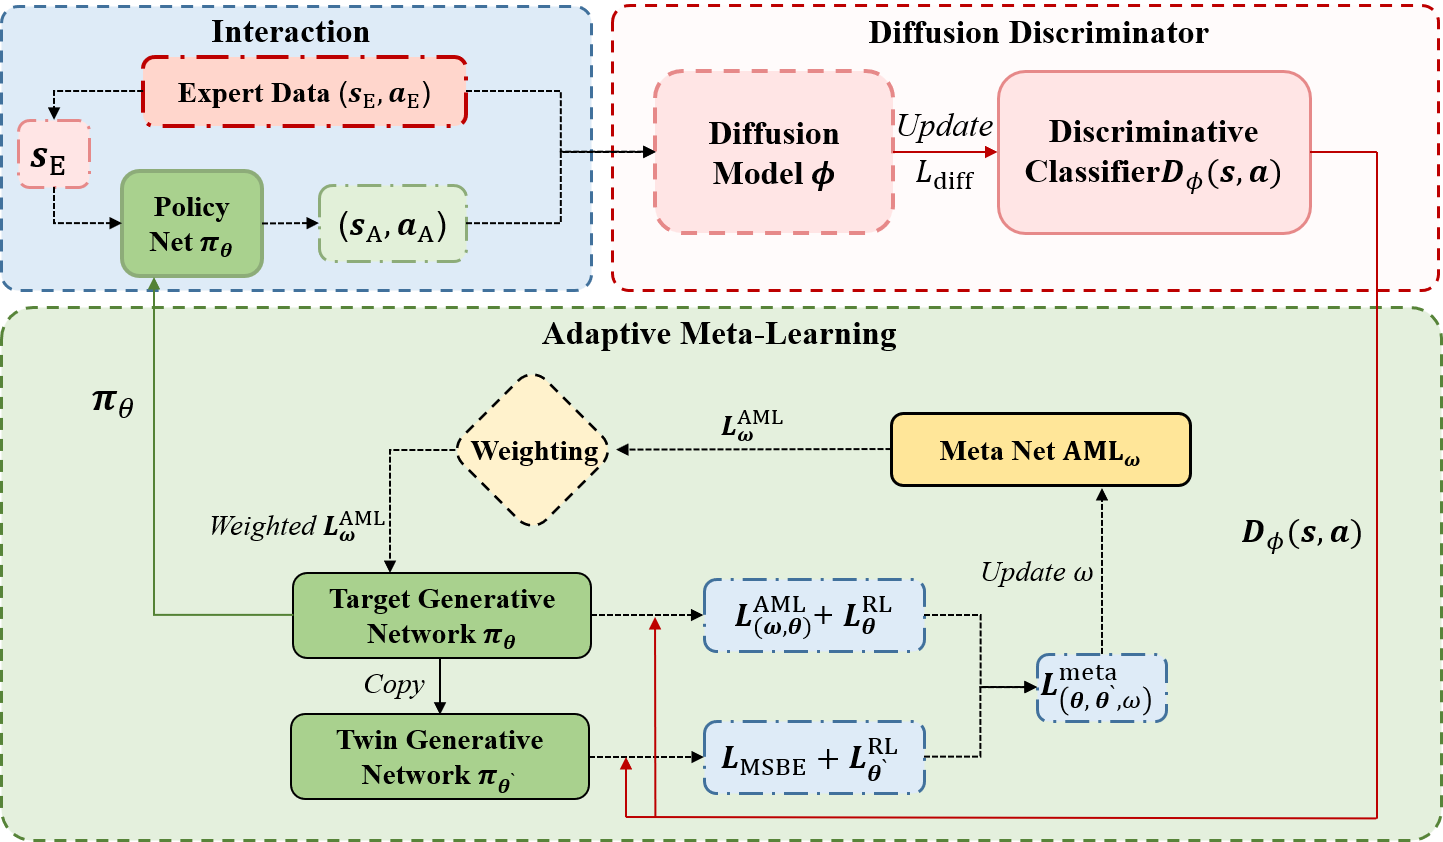
\includegraphics[width=5.5in]{AMLN.png}
\caption{The AMAIL framework consists of three components: policy-environment interaction, a diffusion-based discriminator, and an adaptive meta-generator. Solid lines indicate parameter updates, while dashed lines represent the flow of input and output data. During training, the generator is updated using a normalized reward provided by the discriminator in the interaction phase. This reward replaces the environment reward during rollout, ensuring that learning is guided by discriminator-derived feedback.}
\label{fig_1}
\end{figure*}

\section{Method}
This section presents an Adaptive-Meta Adversarial Imitation Learning (AMAIL) framework designed to improve the training efficiency and stability of diffusion-based adversarial imitation learning. The proposed method is formulated as a bilevel optimization problem, where generalized imitation learning first extracts structured expert knowledge from offline data, which is subsequently integrated into online reinforcement learning to guide policy improvement. To further enhance training stability and sample efficiency, an offline data evaluation mechanism is introduced to dynamically regulate the influence of meta-learning during policy updates.

The AMAIL framework consists of three key components: policy-environment interaction, a diffusion-based discriminator, and an adaptive meta-learning network (AMLN), as illustrated in Fig. \ref{fig_1}. The interaction module generates trajectories and action distributions, which are used both to train the diffusion discriminator and to regulate the meta-learning signal during policy optimization. The diffusion discriminator leverages a denoising process to quantify discrepancies between expert and generated actions by modeling the difference between predicted and injected noise, thereby providing more expressive distribution-level feedback.

Building upon this, the AMLN employs discriminator outputs as reward signals and introduces a hierarchical architecture comprising an upper-level meta-network and a twin generative network. This structure enables the extraction of intrinsic expert behavior patterns, improves data efficiency under limited supervision, and adaptively modulates the influence of meta-learning on policy updates. As a result, the proposed design enhances training robustness while maintaining effective optimization of the target policy network.

\subsection{Diffusion Discriminator}
During policy-environment interaction, rollouts are collected to train a diffusion-based discriminator and to provide imitation-guided supervision for subsequent policy updates. Unlike conventional binary classifiers, the proposed discriminator derives its decision signal from the denoising process of a diffusion model, where the discrepancy between injected noise and predicted noise reflects the degree of consistency between a state-action pair and the target behavior distribution.

Specifically, for a given state-action pair $(s,a)$, a diffusion timestep $t$ is sampled and Gaussian noise $\epsilon$ is injected to construct a corrupted input. The denoising network $\epsilon_\phi(\cdot)$ then takes $(s,a)$, $t$, and the noisy observation as input, conditioned on a label $\kappa$ indicating the data source (expert or agent). The diffusion fitting loss is defined as
\begin{equation}
\label{eq:diff_loss_re}
\mathcal{L}_{\text{diff}}(s,a,\kappa)= \mathbb{E}_{t,\epsilon}\Big[||\epsilon_\phi(s,a,\epsilon,t\mid \kappa)-\epsilon||_2^2\Big]
\end{equation}
where $\kappa$ denotes whether the sample originates from expert demonstrations or agent-generated rollouts. The loss under the expert condition measures alignment with expert behavior, while the loss under the agent condition quantifies deviation from the learned policy distribution.

To obtain a stable and bounded learning signal, the unnormalized diffusion losses are transformed into a discriminative score defined as
\begin{equation}
  \label{eq:discriminator}
  D_\phi(s,a)=\sigma\left(\mathcal{L}_{\text{diff}}(s,a,\kappa_{\text{agent}}) -\mathcal{L}_{\text{diff}}(s,a,\kappa_{\text{expert}})\right)
\end{equation}
where $\sigma(\cdot)$ denotes the sigmoid function. This formulation produces a bounded estimate of expert-likeness, where higher values indicate closer alignment with expert behavior.

The discriminator is optimized using a binary cross-entropy objective, where diffusion losses computed from expert demonstrations and policy rollouts are used to form classification targets. Through iterative updates, $D_\phi$ learns to distinguish expert and agent distributions based on denoising discrepancy rather than direct binary classification. The resulting output provides a stable, distribution-aware reward signal for downstream policy optimization, thereby alleviating the instability commonly associated with minimax adversarial training.

\subsection{On-Policy Adaptive Meta-Learning Network}

The adaptive meta-learning mechanism is implemented via a dual-layer architecture. During policy updates, the target policy network $\pi_\theta$ is duplicated to construct a temporary twin network $\pi_{\theta'}$. These two networks correspond to the lower-level learner and the upper-level meta-learner, respectively, and are connected through differentiable parameter dependencies, enabling bilevel optimization.

The lower-level network is optimized using trajectories and rewards collected from environment interactions. To improve learning efficiency, gradient signals from both imitation learning (IL) and adaptive meta-learning (AML) are incorporated. After independent updates, performance discrepancies emerge between the twin network (optimized with RL+IL) and the target network (optimized with RL+AML). The upper-level meta-network captures this performance gap, which reflects the advantage of incorporating AML, and uses it as a learning signal for meta-optimization.

The lower-level optimization follows the proximal policy optimization (PPO) framework. Rollout data are used to compute discounted returns and advantage estimates, followed by multiple epochs of stochastic updates. For each batch, the target network is first cloned to form the twin network, which is optimized using a hybrid reinforcement learning and imitation learning objective. The clipped policy loss is defined as
\begin{flalign}
  \label{Agent_loss}
  &\qquad L^{\prime}_{\text{CLIP}}=E[\text{min}(\varDelta_{\ell(\theta)} \cdot A_{\pi}(s,a), \nonumber&\\
  &\quad \quad \quad\quad \quad\quad \quad\text{clip}(\varDelta_{\ell(\theta)},1-\epsilon ,1+\epsilon )\cdot A_{\pi}(s,a))].&
\end{flalign}
where $\varDelta_{\ell(\theta)}$ denotes the probability ratio between the new and old policies, and $A_{\pi}(s,a)$ is the advantage estimate computed from discounted returns.

To stabilize value estimation, the critic is regularized using a clipped mean-squared error objective:
\begin{equation}
\label{Value_loss}
V^{\prime}_{\text{loss}}=\frac{1}{2}\text{max}[(V^{\prime}-r)^2,(V^{\prime}_{\text{clip}}-r)^2]
\end{equation}

Behavior cloning is further incorporated using expert samples within the same batch, yielding the combined twin-network objective:
\begin{equation}
\label{tmp_loss}
L^{\prime} = L^{\prime}_{a} + c_{\text{v}} \cdot V^{\prime}_{\text{loss}} + c_{\text{bc}} \cdot L^{\text{BC}} - c_{\text{ent}} \cdot \mathbb{E}[H^{\prime}(x_{\theta^{\prime}})]
\end{equation}
where $c_\text{v}$, $c_{\text{bc}}$, and $c_{\text{ent}}$ are weighting coefficients. This objective is used to update the twin network and serves as a reference baseline for meta-learning.

Subsequently, the target policy network is optimized using both reinforcement learning and AML signals. In addition to the standard PPO objective, an AML loss is introduced. Specifically, the AML module consumes state–action pairs generated by the target policy to compute an initial meta-guided loss, which is then reweighted by the discriminator-derived importance signal $W$. The resulting AML objective is defined as
\begin{equation}
  L^{\text{AML}}_{(\omega,\theta)}=\mathbb{E}[f_{\text{AML}}\cdot W]
\end{equation}
The overall optimization objective of the target policy becomes
\begin{equation}
\label{actor_loss}
  L = L_{a} + c_{\text{v}} \cdot V_{\text{loss}} + L^{\text{AML}}_{(\omega,\theta)} - c_{\text{ent}} \cdot \mathbb{E}[H(x_{\theta})]
\end{equation}
During the lower-level update, the AMLN receives state-action pairs $(s^d, a^d)$ from demonstrations and the corresponding policy-generated actions $a = \pi_\theta(s^d)$ as inputs. To update the upper-level AMLN, the meta-objective must remain differentiable with respect to its parameters $\omega$, enabling gradient propagation through the bilevel structure.

The upper-level objective quantifies the performance gap between the twin network and the target network:
\begin{equation}
\label{AMLN_loss}
L^{\text{meta}}_{(\theta,\theta^{\prime},\omega)}= \text{tanh}(L_{\pi_{\theta^{\prime}}}-L_{\pi_{\theta}})
\end{equation}
where $L_{\pi_{\theta^{\prime}}}$ denotes the loss of the twin policy (RL+IL), and $L_{\pi_{\theta}}$ denotes the loss of the target policy (RL+AML). The AMLN is then updated by minimizing the negative of this objective, thereby reinforcing configurations in which AML-enhanced policies outperform pure imitation-guided updates.
\begin{algorithm}[H]
\caption{algorithm of AMLN}\label{alg:AML}
\begin{algorithmic}[1]
\REQUIRE Policy network $\pi_\theta$, Discriminator $D_\phi$, AMAIL network $G_\omega$, Expert demonstrations $\mathcal{D}_E$, Rollouts $\mathcal{R}$
\ENSURE Optimized policy network $\pi_{\theta^\star}$, Learned AML network $G_{\omega^\star}$
\STATE \textbf{for} $epoch = 1,2,...,N_{epochs}$ \textbf{do}
\STATE \hspace{0.5cm}Sample mini-batches $\mathcal{B} \sim \mathcal{R} $
\STATE \hspace{0.5cm}\textbf{for} each mini-batch $\mathcal{B}$ \textbf{do}
\STATE \hspace{1cm}Clone policy: $\theta^{\prime}\leftarrow \theta$
\STATE \hspace{1cm}Calculate PPO surrogate loss via Eq. \eqref{Agent_loss}
\STATE \hspace{1cm}Calculate clipped value loss via Eq. \eqref{Value_loss}
\STATE \hspace{1cm}Sample expert data $(s_E,a_E) \sim \mathcal{D}_E$
\STATE \hspace{1cm}Calculate behavior loss $L^{\text{BC}}=\lVert \pi_{\theta^{\prime}}(s_E)-a_E \rVert_2^2$
\STATE \hspace{1cm}Update the twin network using loss $L^{\prime}$ via Eq. \eqref{tmp_loss}
\STATE \hspace{1cm}Evaluate PPO loss using $\pi_{\theta}$
\STATE \hspace{1cm}Generate policy actions $a_\theta=\pi_\theta(s_E)$
\STATE \hspace{1cm}Calculate AMLN output $f_{AML}([a_\theta,s_E,a_E])$
\STATE \hspace{1cm}Calculate total policy loss via Eq. \eqref{actor_loss}
\STATE \hspace{1cm}Update policy network $\theta$ using loss $L$
\STATE \hspace{1cm}Update AMLN via Eq. \eqref{AMLN_loss}
\STATE \hspace{0.5cm}\textbf{end for}
\STATE \textbf{end for}
\end{algorithmic}
\label{alg1}
\end{algorithm}
\subsection{Adaptive Learning Weights}
In our architecture, the upper-level AMLN provides supervisory signals that can be interpreted as an enhanced form of imitation learning. Specifically, the objective is to learn a policy $\pi_\theta(a \mid s)$ that approximates the expert policy $\pi_E(a \mid s)$ from demonstration data. As with standard imitation learning, this paradigm inevitably inherits two fundamental limitations: strong dependence on expert demonstrations and vulnerability to distributional shift. When demonstrations are noisy or suboptimal, compounding errors may arise, leading to exponential performance degradation over long horizons.

Within adversarial imitation learning, moderate demonstration noise may induce a regularization effect by smoothing the discriminator’s decision boundary. However, excessive noise deteriorates the discriminator's ability to distinguish correct behavioral patterns, resulting in unstable policy updates and directional drift. To alleviate this issue, we introduce confidence-based adaptive weighting, where samples with higher uncertainty or noise are down-weighted, thereby reducing their adverse impact on policy optimization.

To formalize this weighting mechanism, we relate it to performance improvement in reinforcement learning. For a policy $\pi$, its expected discounted return under a Markov decision process (MDP) is defined as

\begin{equation}
\eta (\pi)=\mathbb{E}_{\pi} \left[ \sum_{t=0}^{T} \gamma^t r(s_t,a_t) \right]
\end{equation}

The performance difference between two policies $\widetilde{\pi}$ and $\pi$ can be characterized by $\eta(\widetilde{\pi}) - \eta(\pi)$. Since directly sampling from $\pi$ may be impractical, we instead consider the surrogate objective

\begin{equation}
  L^{d_{\pi}}(\widetilde{\pi})=\sum_{s} d_{\pi}(s) \sum_{a} \widetilde{\pi}(a|s) A_{\pi}(s,a)
\end{equation}

where $d_{\pi(s)}=\mathbb{E}[\sum_{t=0}^{T} \gamma^t \mathbf{1}(s_t=s)]$ denotes the discounted state visitation distribution of $\pi$, and $A_\pi(s,a)$ is the advantage function.

To ensure policy improvement while preventing excessive deviation from the reference policy, we introduce an $f$-divergence regularization over occupancy measures:

\begin{equation}
  \max_{\widetilde{\pi}}\quad  L^{d_{\pi}}(\widetilde{\pi}) - \beta D_{f}\!\big(\rho_{\tilde{\pi}}\|\rho_{\pi}\big) ,
	\quad \text{s.t.} \sum_{a}\widetilde{\pi}(a\mid s)=1
\end{equation}
Here, $\beta > 0$ controls the trade-off between performance maximization and distributional proximity to $\pi$. Solving this constrained optimization problem via Lagrangian duality yields

\begin{equation}
  \widetilde{\pi}(a \mid s)=\pi(a \mid s) f_{*}^{\prime}\left(\frac{1}{\beta}\left(A_{\pi}(s, a)+C(s)\right)\right)
\end{equation}
where $f^*$ denotes the convex conjugate of $f$. Under the KL-divergence instantiation, the solution reduces to an exponential reweighting:
\begin{equation}
  \widetilde{\pi}(a \mid s)=\pi(a \mid s) \exp \left(\frac{1}{\beta}\left(A_{\pi}(s, a)+C(s)\right)\right)
\end{equation}
Consequently, the corresponding occupancy measure satisfies
\begin{equation}
  \rho_{\widetilde{\pi}}(s, a)=\rho_{\pi}(s, a) \exp \left(\frac{1}{\beta}A_{\pi}(s, a)\right)
\end{equation}
Analogous to weighted GAIL (WGAIL), we define a multiplicative weight function $\omega(s,a)$ such that
\begin{equation}
  \rho_{\widetilde{\pi}}(s, a)= \omega(s, a)\rho_{\pi}(s, a) 
\end{equation}
which implies $\omega \propto A_\pi$. Therefore, adaptive weighting is theoretically grounded in advantage-based policy improvement.

In practice, however, the true advantage function is not directly accessible. To approximate $\omega(s,a)$, we exploit the diffusion discriminator. Let $\mathcal{L}_{\text{diff}}(s,a,c)$ denote the diffusion loss under condition $c$, where $c^+$ corresponds to expert data and $c^-$ to agent-generated data. The discriminator output is defined as

\begin{flalign}
D_{\phi}(s,a) &= \frac{e^{-\mathcal{L}_{\text{diff}}(s,a,c^+)}}{e^{-\mathcal{L}_{\text{diff}}(s,a,c^+)}+e^{-\mathcal{L}_{\text{diff}}(s,a,c^-)}} \notag\\
&= \sigma(\mathcal{L}_{\text{diff}}(s,a,c^-)-\mathcal{L}_{\text{diff}}(s,a,c^+)) \notag\\
&= \frac{\pi_{\theta}(a\mid s)}{\pi_{\theta}(a\mid s)+\omega(s,a)\pi(a \mid s)} \notag \\
&= \frac{\pi_\theta(a \mid s)}{\pi_\theta(a \mid s)+\omega(s , a)\text{exp}(A_\pi (s,a))}
\end{flalign}

Following the adversarial learning formulation of Fu et al., the discriminator implicitly recovers the log-density ratio between expert and policy distributions. Leveraging this relationship, we express the optimal discriminator as

\begin{equation}
D_{\psi }^{\ast }(s,a)=\frac{\pi_\theta(a \mid s)}{\pi_\theta(a \mid s)+\omega(s,a)^{(\beta+1)}}
\end{equation}

Solving for $\omega(s,a)$ yields

\begin{equation}
  \omega(s,a)=\left[\left(\frac{1}{D_\psi ^{\ast }(s,a)}-1\right)\pi_\theta(a \mid s)\right]^{\frac{1}{\beta+1}}
\end{equation}

This formulation enables us to compute adaptive sample weights directly from the diffusion discriminator output. The resulting weighted AML objective attenuates the influence of noisy or low-confidence demonstrations, thereby mitigating error accumulation and improving robustness under suboptimal expert data and environmental perturbations.

\begin{figure*}[!t]
\centering

\subfloat[FETCHPUSH]{%
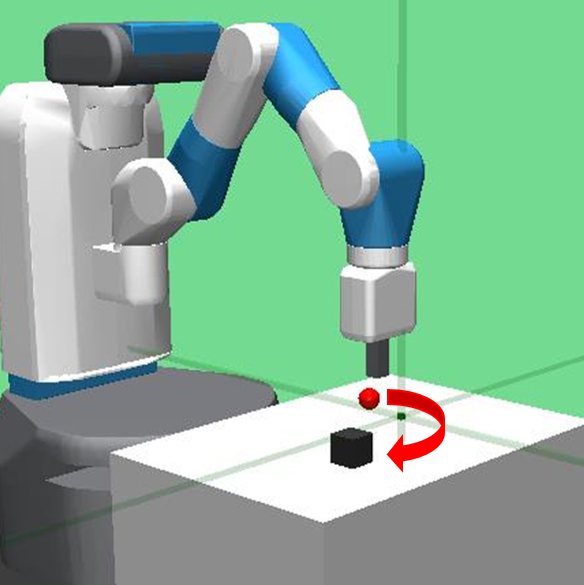
\includegraphics[width=0.16\textwidth]{pic1}%
\label{fig_first_case}}%
\hfill
\subfloat[FETCHPICK]{%
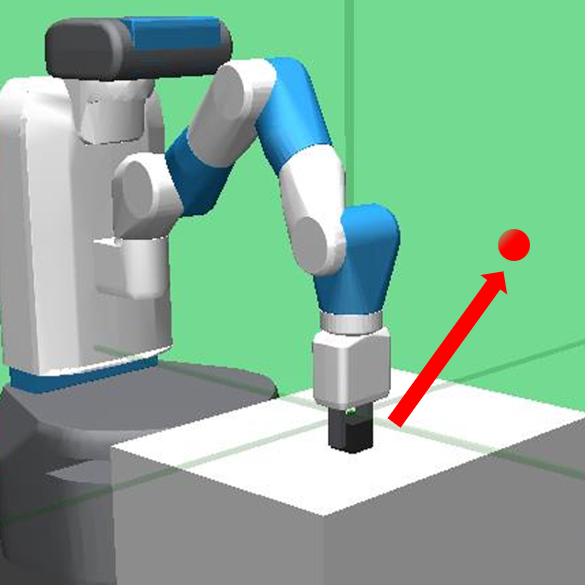
\includegraphics[width=0.16\textwidth]{pic2}%
\label{fig_second_case}}%
\hfill
\subfloat[ANTREACH]{%
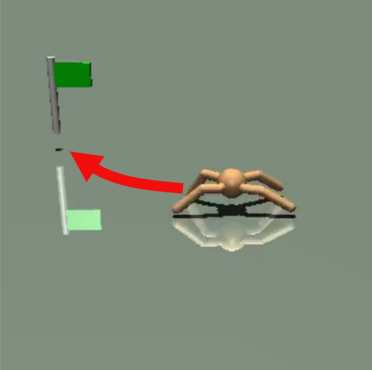
\includegraphics[width=0.16\textwidth]{pic3}%
\label{fig_third_case}}%
\hfill
\subfloat[HANDROTATE]{%
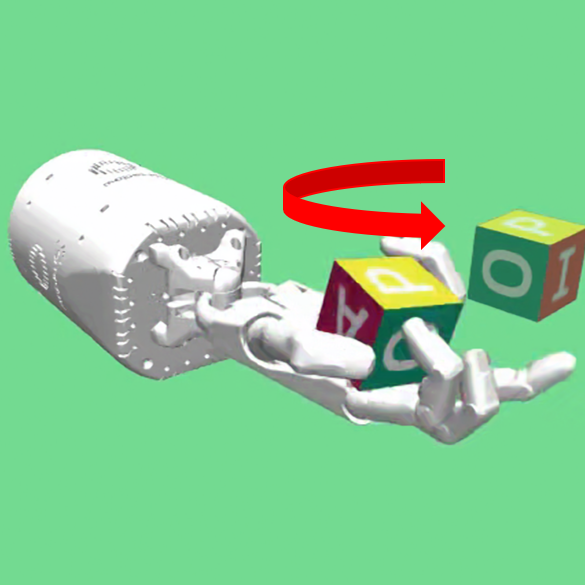
\includegraphics[width=0.16\textwidth]{pic4}%
\label{fig_fourth_case}}%
\hfill
\subfloat[MAZE]{%
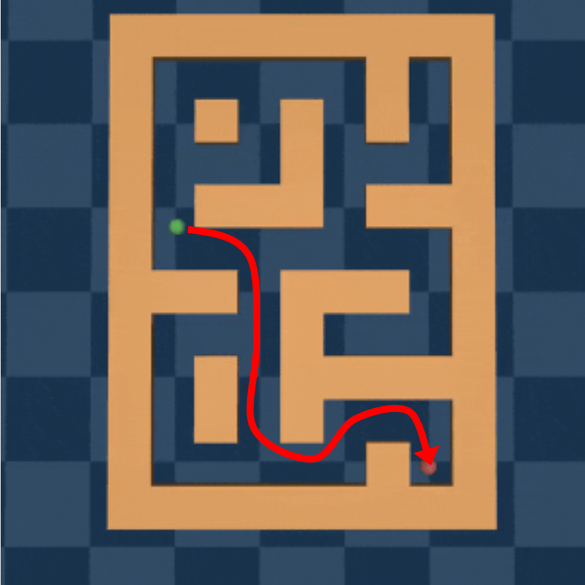
\includegraphics[width=0.16\textwidth]{pic5}%
\label{fig_fifth_case}}%
\hfill
\subfloat[WALKER]{%
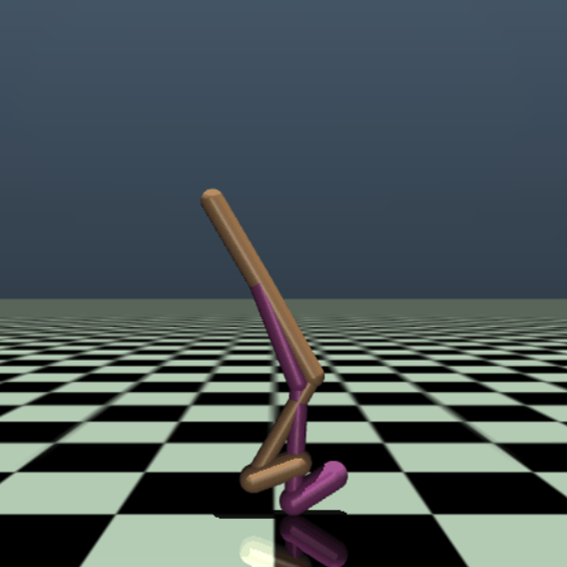
\includegraphics[width=0.16\textwidth]{pic6}%
\label{fig_sixth_case}}%

\caption{The experiments mainly consist of five goal-oriented tasks and one performance-oriented task. (a) The robotic arm needs to push the object to the target point. (b) The robotic arm needs to pick up the object and move it to the target point. (c) The ant agent needs to move to the target point indicated by the flag. (d) The dexterous hand needs to rotate the cube in its hand to the target direction. (e) The agent needs to pass through the maze from the green starting point to reach the red target point. (f) The bipedal walker needs to move forward as far as possible within a fixed time.}
\label{fig_sim}
\end{figure*}


\section{Experiment}

This section evaluates the performance and data utilization of the proposed AMAIL, demonstrating its superiority in a random environment, as well as its improvements in training efficiency and generalization compared to existing methods. The proposed framework has been extensively evaluated in various continuous control domains, including navigation, robotic arm operation, and motion, all of which were conducted on the MuJoCo platform. To prove the improved performance and expert sample utilization of the proposed method, the environment scenarios were expanded according to the settings described by Lee et al.
\subsection{Simulation setup}
This section describes the benchmark environments, task configurations, and expert datasets used to evaluate AMAIL.

\textbf{FETCHPUSH.} We first evaluate AMAIL on the 7-DoF FetchPush manipulation task (Fig. 3a), where a robotic arm must push a block to a target location indicated by a red marker. The 16-dimensional observation vector comprises the gripper pose, object pose, relative gripper-object pose, and goal position. Both the initial object configuration and target position are randomized across episodes. We adopt the expert dataset provided by Lee et al., consisting of 20,311 transitions from 664 trajectories. To assess robustness, Gaussian noise is injected into the initial and goal positions during training.

\textbf{FETCHPICK.} In the FetchPick task (Fig. 3b), the agent must grasp a block and lift it to a designated target location in 3D space. The observation structure is identical to that of FetchPush. We utilize a dataset containing 50,000 transitions generated by a scripted expert policy. As in FetchPush, additional noise is applied to the initial and target block positions during training to evaluate noise tolerance and generalization capability.

\textbf{ANTREACH.} We further evaluate AMAIL on AntReach (Fig. 3c), a high-dimensional locomotion benchmark. In this task, a quadruped ant robot must navigate to a randomly generated target positioned along the boundary of a semicircle with a 5-meter radius centered at the agent. The 132-dimensional state vector encodes joint angles, joint velocities, contact forces, and the goal location relative to the agent. The expert dataset from Lee et al. contains 1,000 demonstration trajectories. To test generalization, random environmental disturbances are introduced during policy training.

\textbf{HANDROTATE.} HandRotate (Fig. 3d) is a challenging dexterous manipulation task involving a 24-DoF Shadow Dexterous Hand. The objective is to rotate a block in-hand to match a specified target orientation. The task features a 68-dimensional state space and a 20-dimensional continuous action space. Observations include joint angles, joint velocities, object pose, and target rotation. We employ an expert dataset collected by Lee et al., consisting of 515 trajectories (approximately 10,000 transitions).

\textbf{MAZE.} We evaluate AMAIL on the MAZE navigation task (Fig. 3e) introduced by Fu et al. In this environment, a point-mass agent must navigate from a randomly sampled start position to a fixed goal location. The agent observes its position and velocity and outputs continuous control signals corresponding to target velocities in the horizontal plane. We use the expert dataset provided by Lee et al., which contains 100 demonstration trajectories (18,525 transitions).

\textbf{WALKER.} We also evaluate AMAIL on the Walker task (Fig. 3f), where a planar bipedal agent is required to walk forward while maintaining balance. The 17-dimensional state includes joint angles, velocities, and body posture, and the 6-dimensional action space outputs continuous joint controls. We use the expert dataset collected by Li et al., containing 1,000 trajectories, and introduce random perturbations during training to assess robustness and generalization.



\begin{figure*}[!t]
\centering

\subfloat[FETCHPUSH]{%
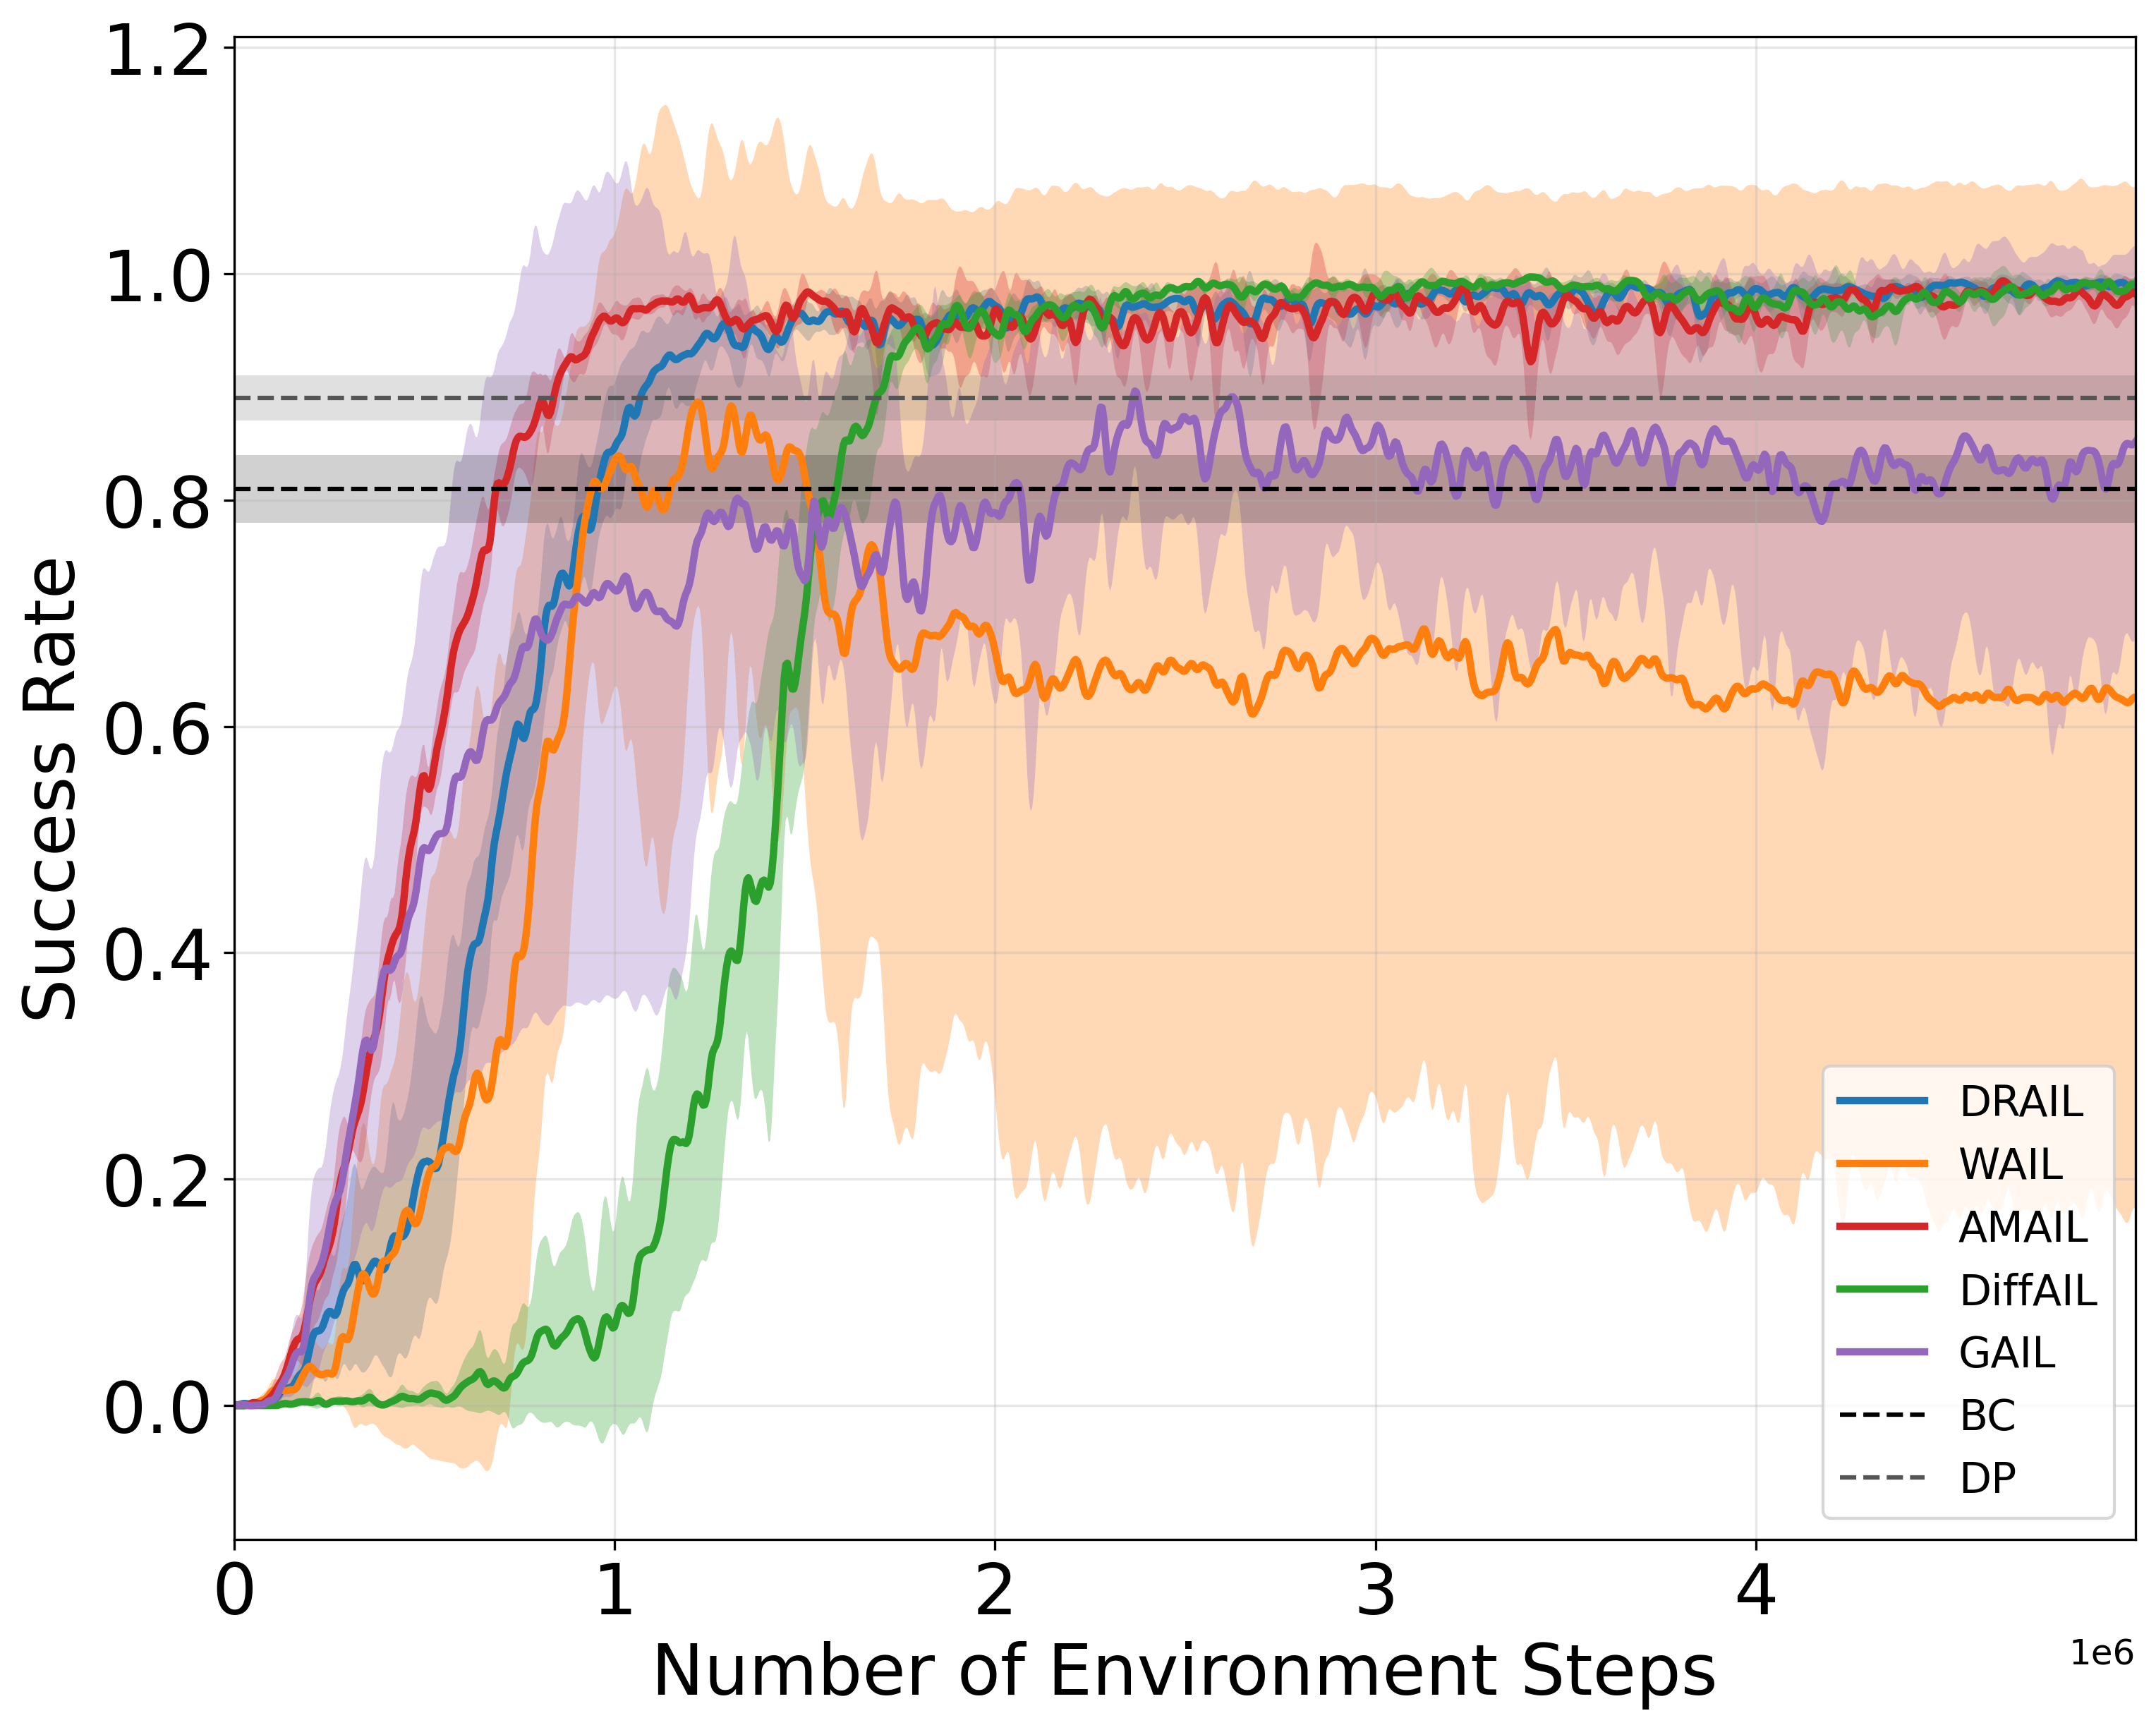
\includegraphics[width=0.33\textwidth]{fetchpush.png}%
\label{fetchpush}}%
\hfill
\subfloat[FETCHPICK]{%
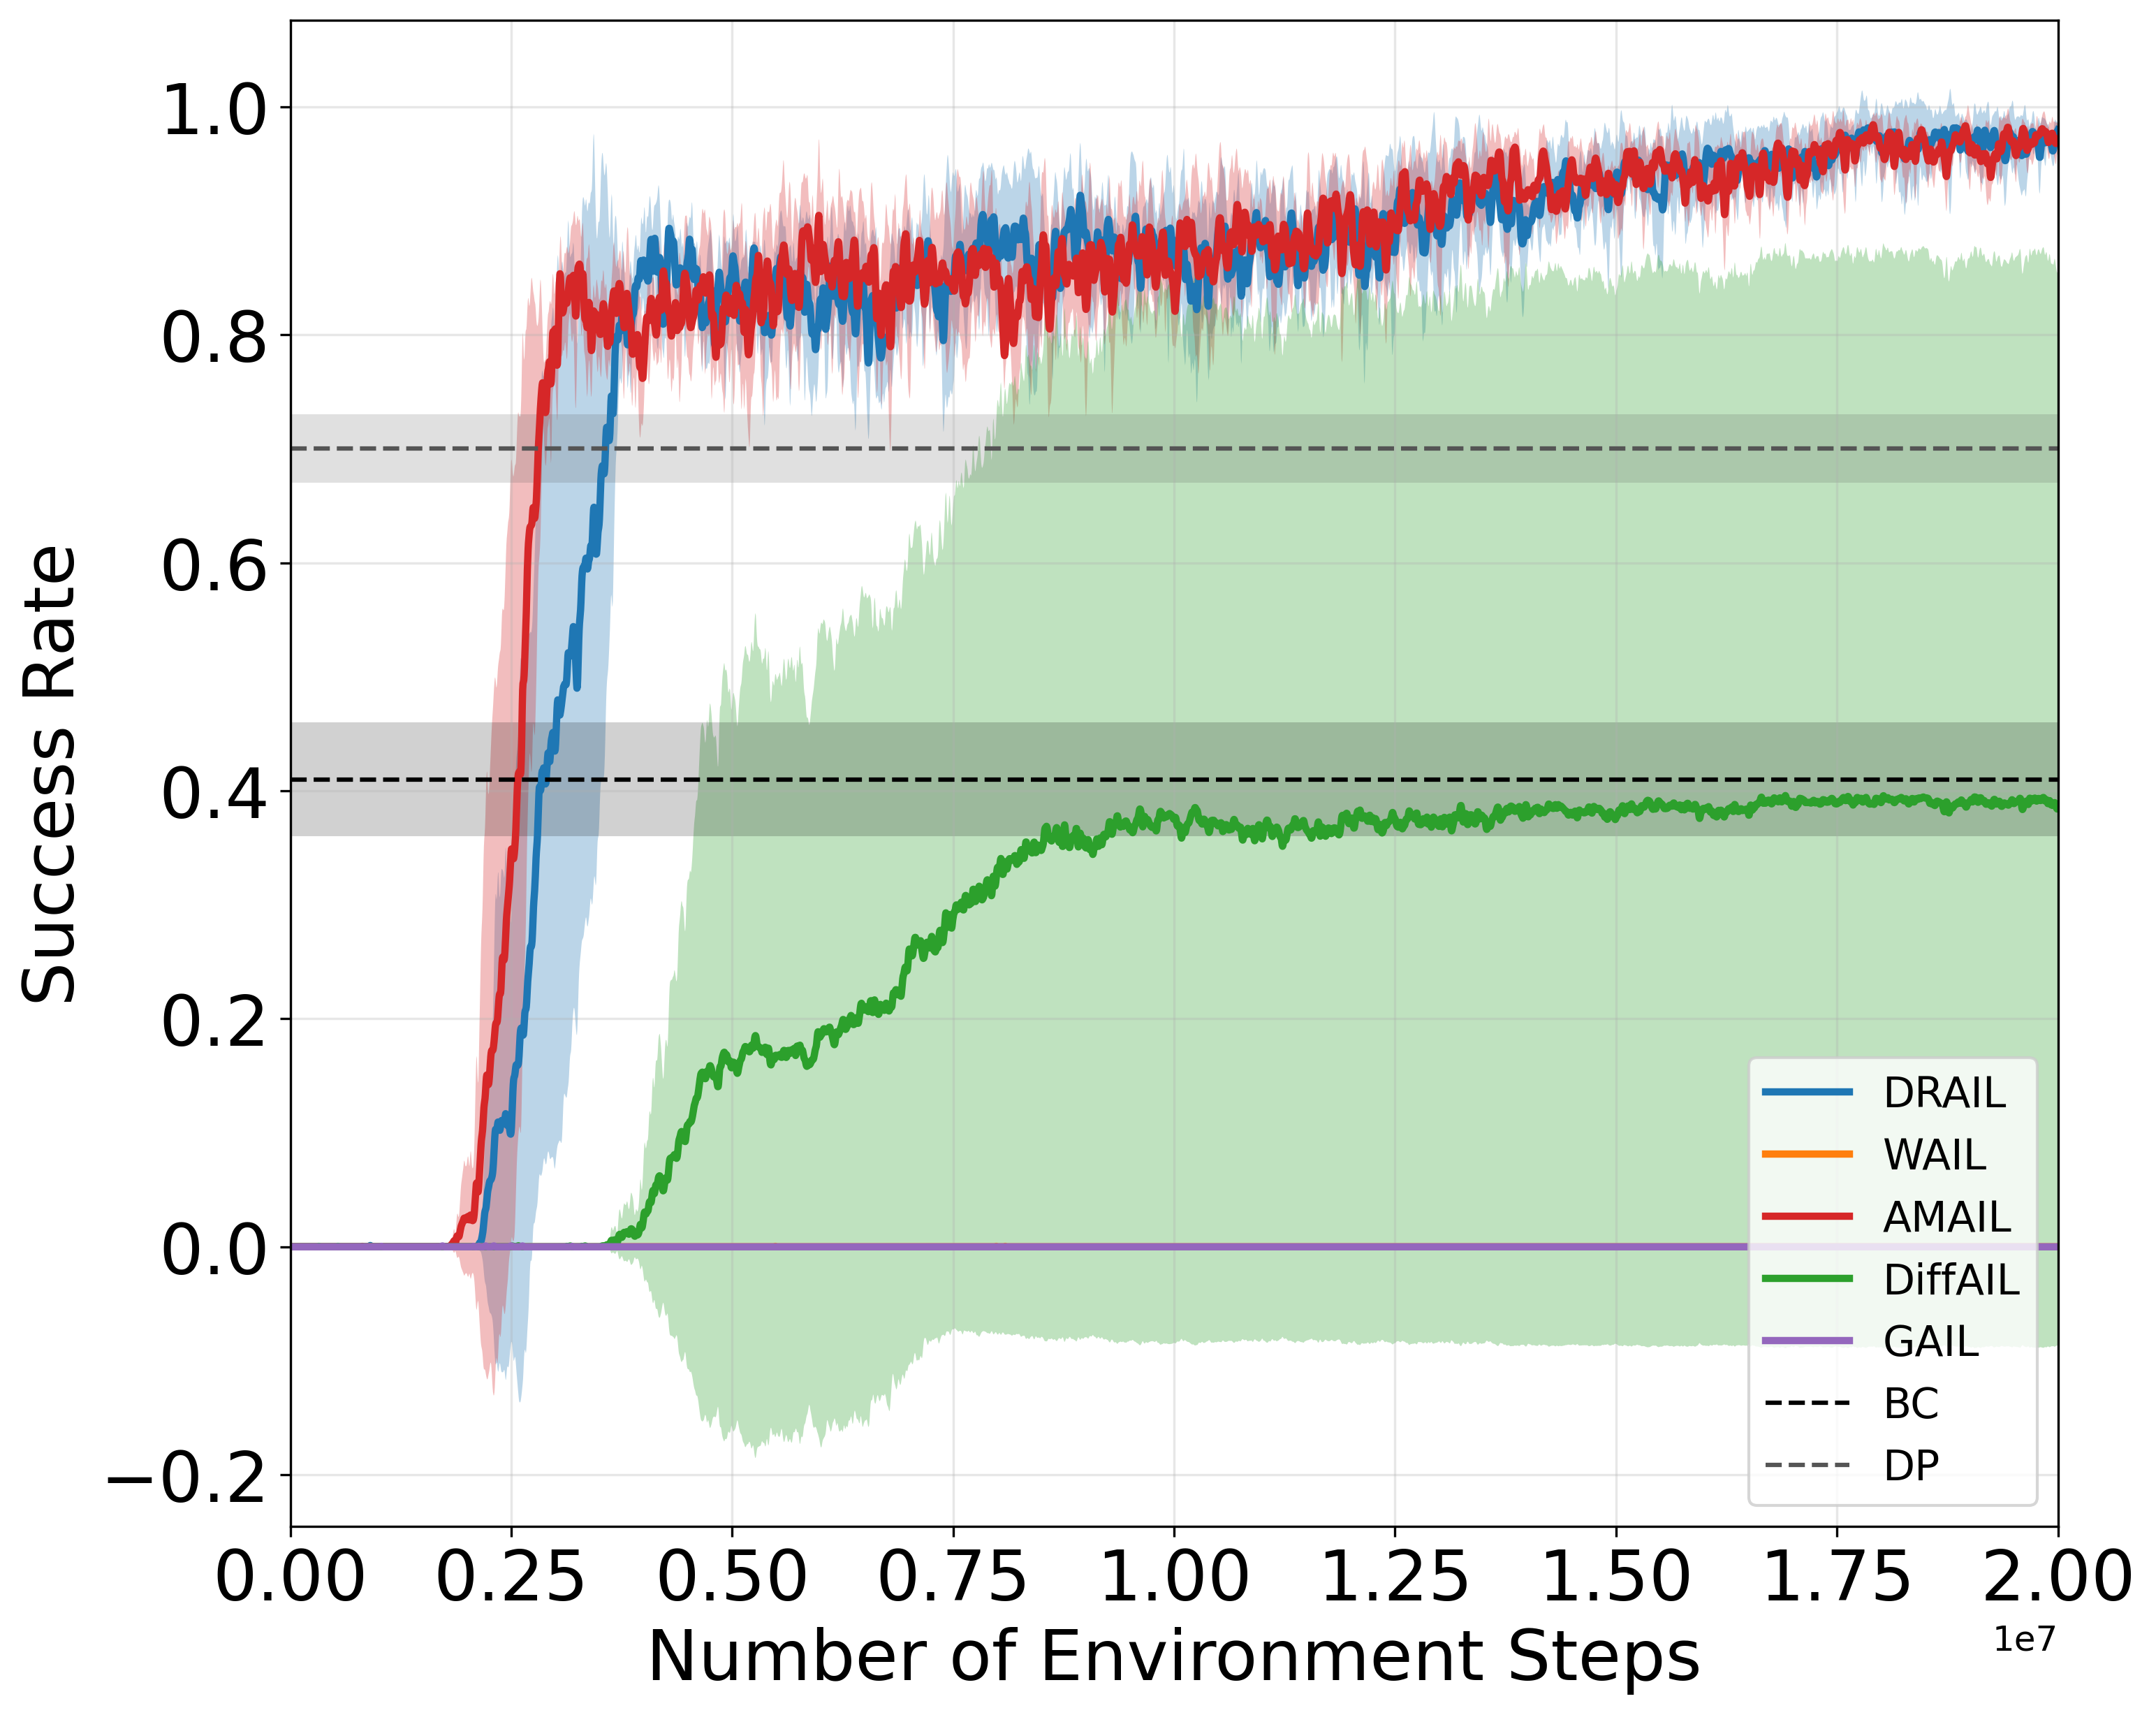
\includegraphics[width=0.33\textwidth]{fetchpick.png}%
\label{fetchpick}}%
\hfill
\subfloat[ANTREACH]{%
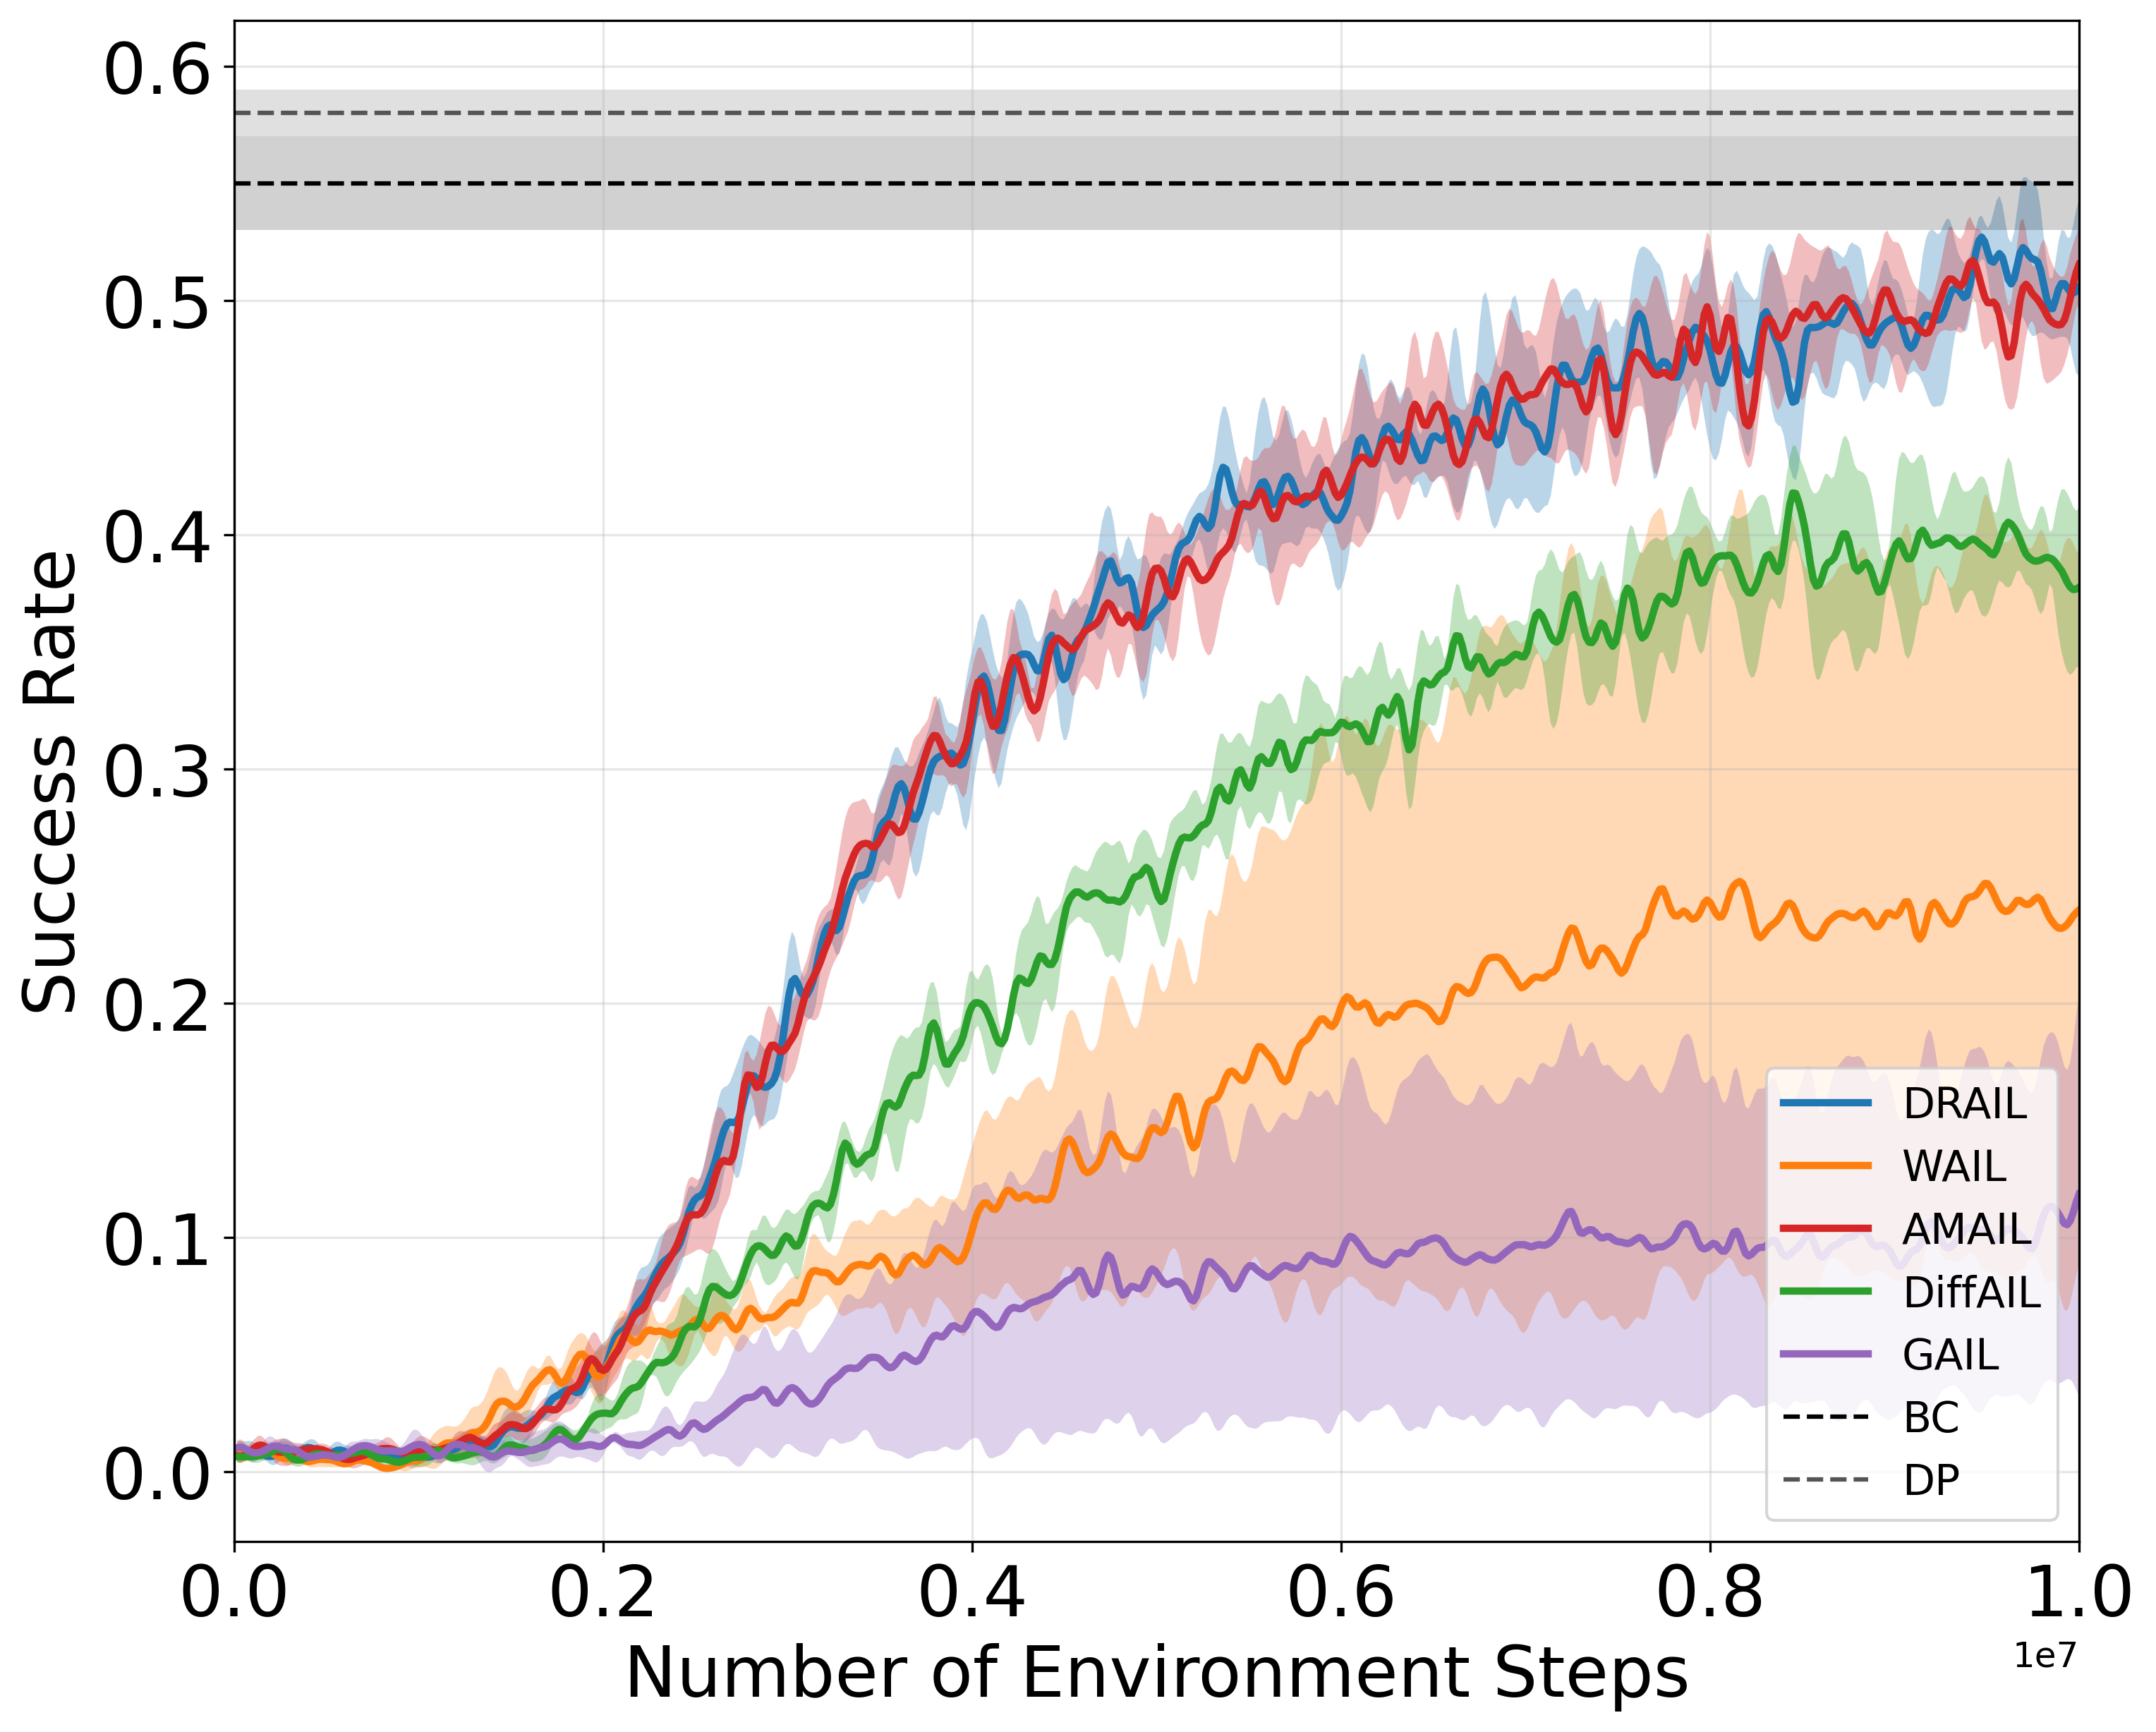
\includegraphics[width=0.33\textwidth]{Antgoal.png}%
\label{antreach}}%
\hfill
\subfloat[HANDROTATE]{%
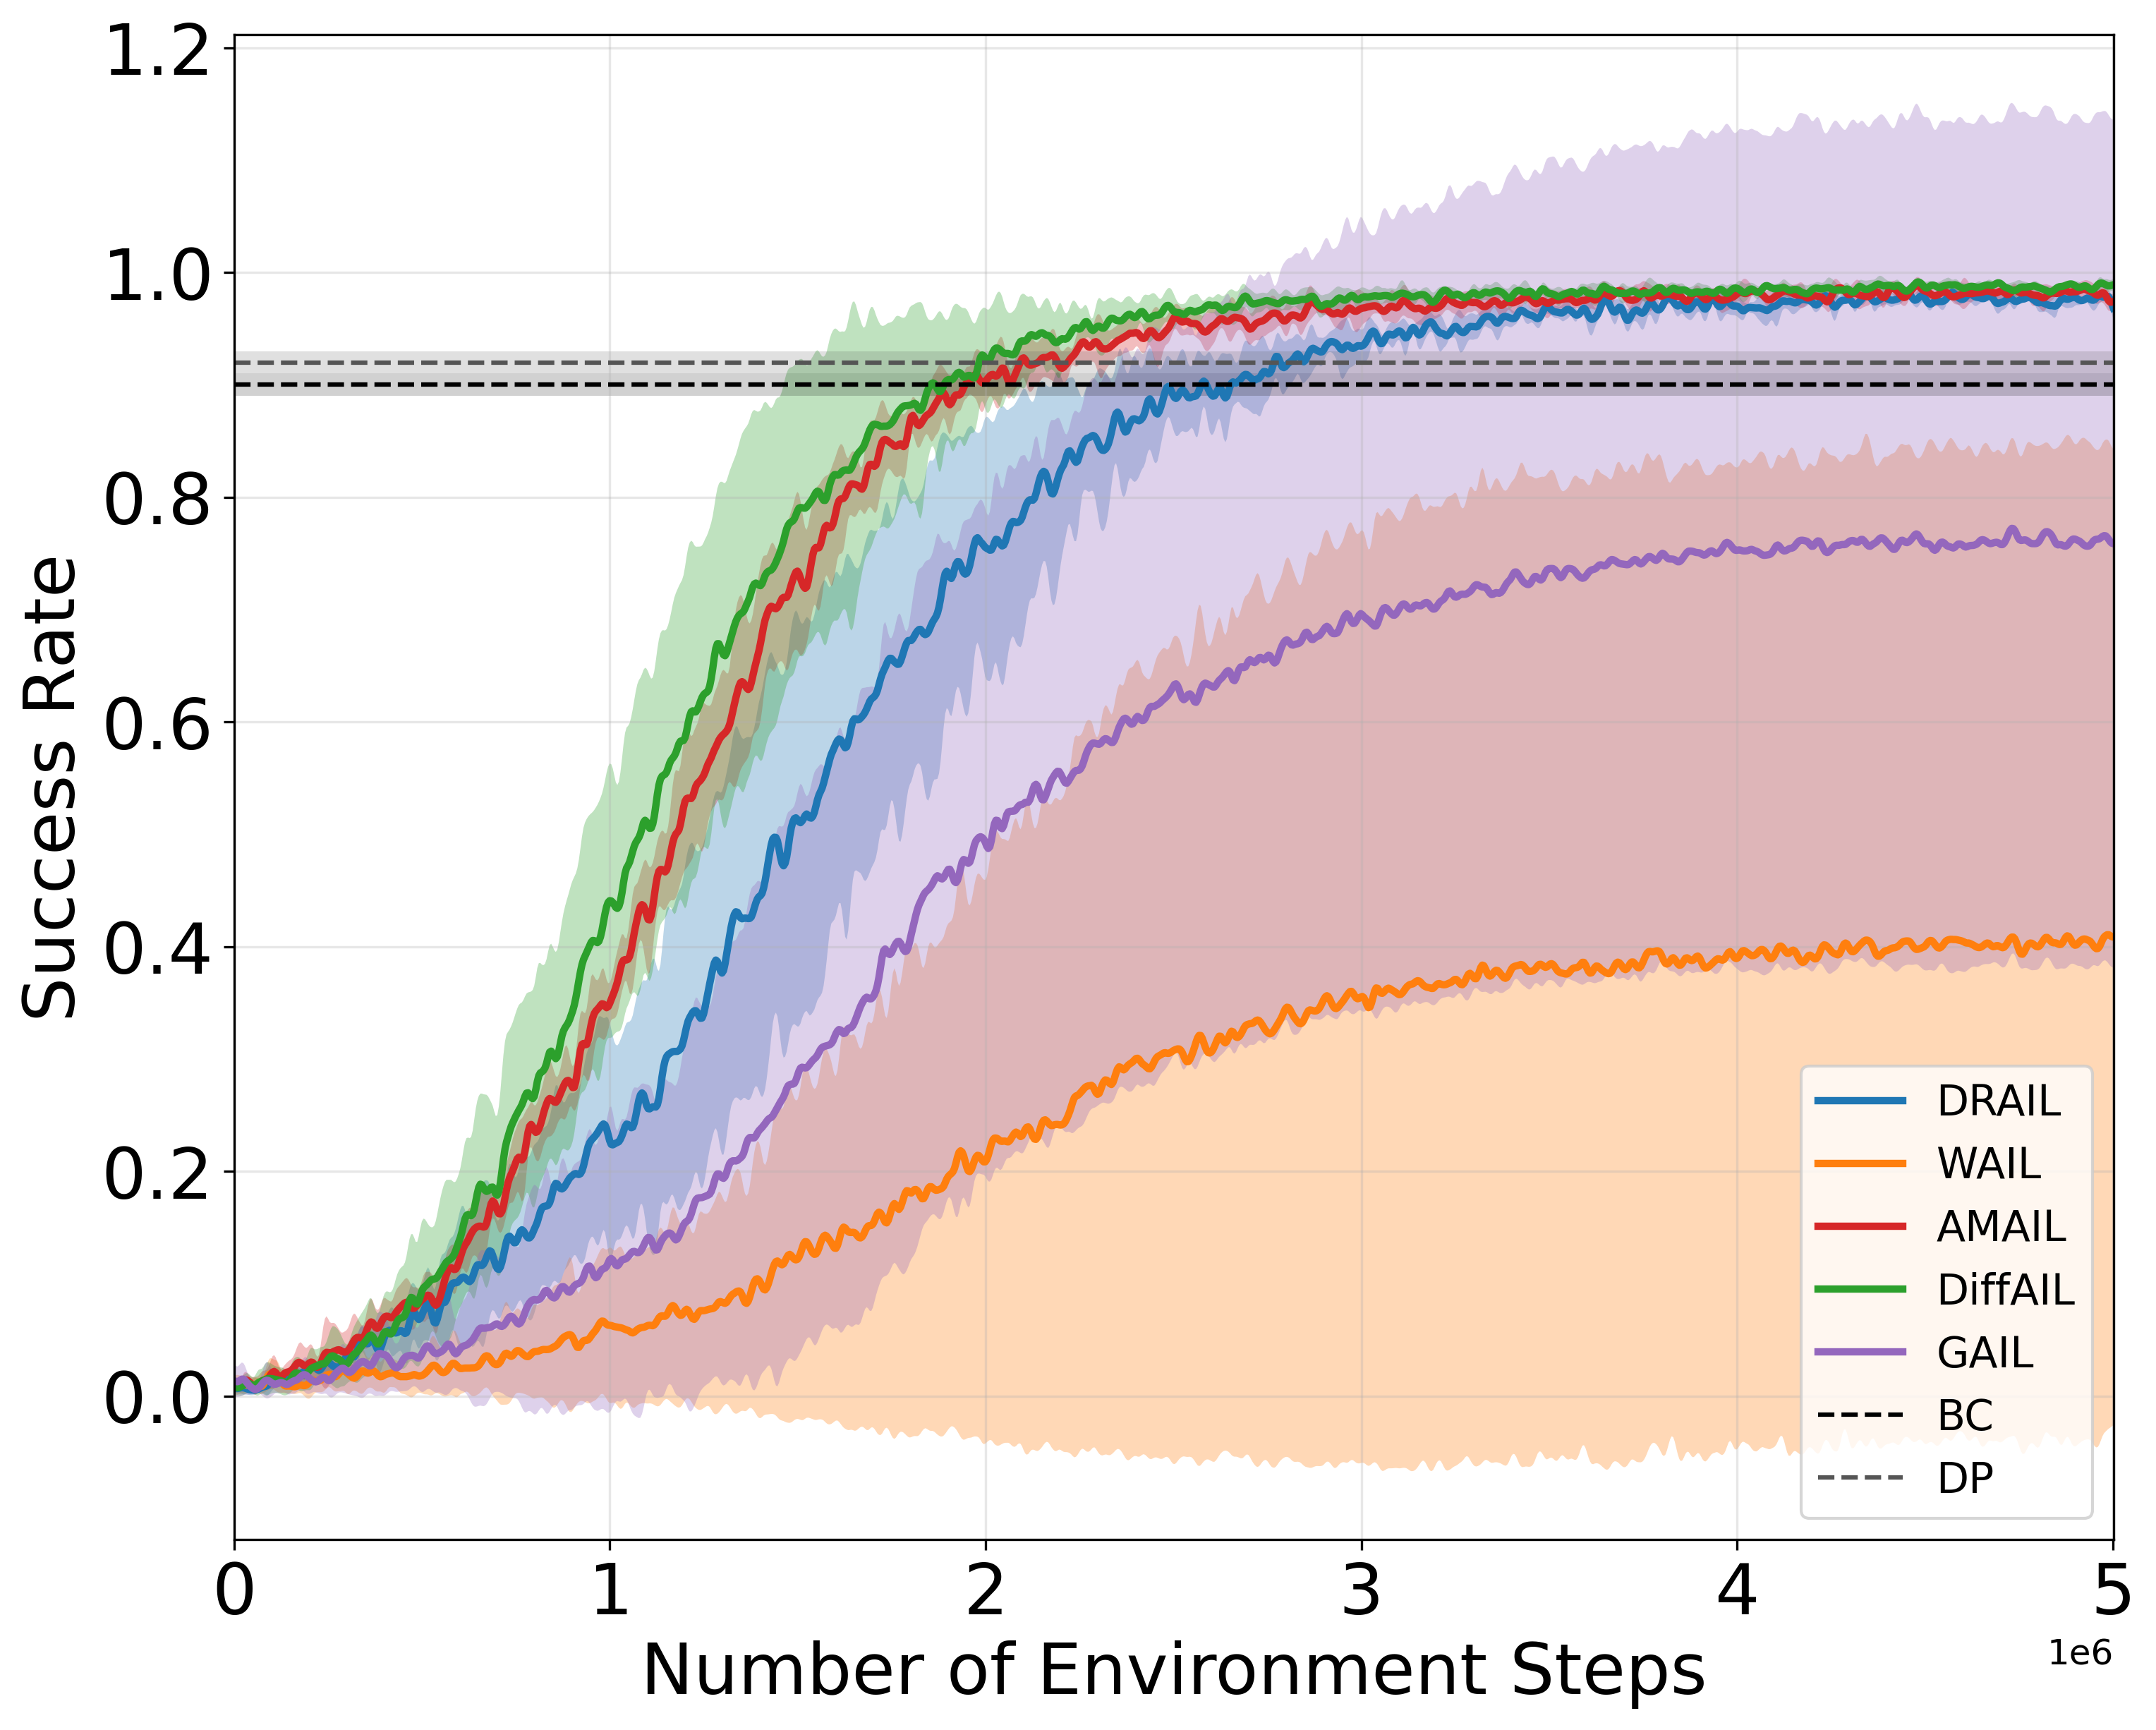
\includegraphics[width=0.33\textwidth]{Hand.png}%
\label{Hand}}%
\hfill
\subfloat[MAZE]{%
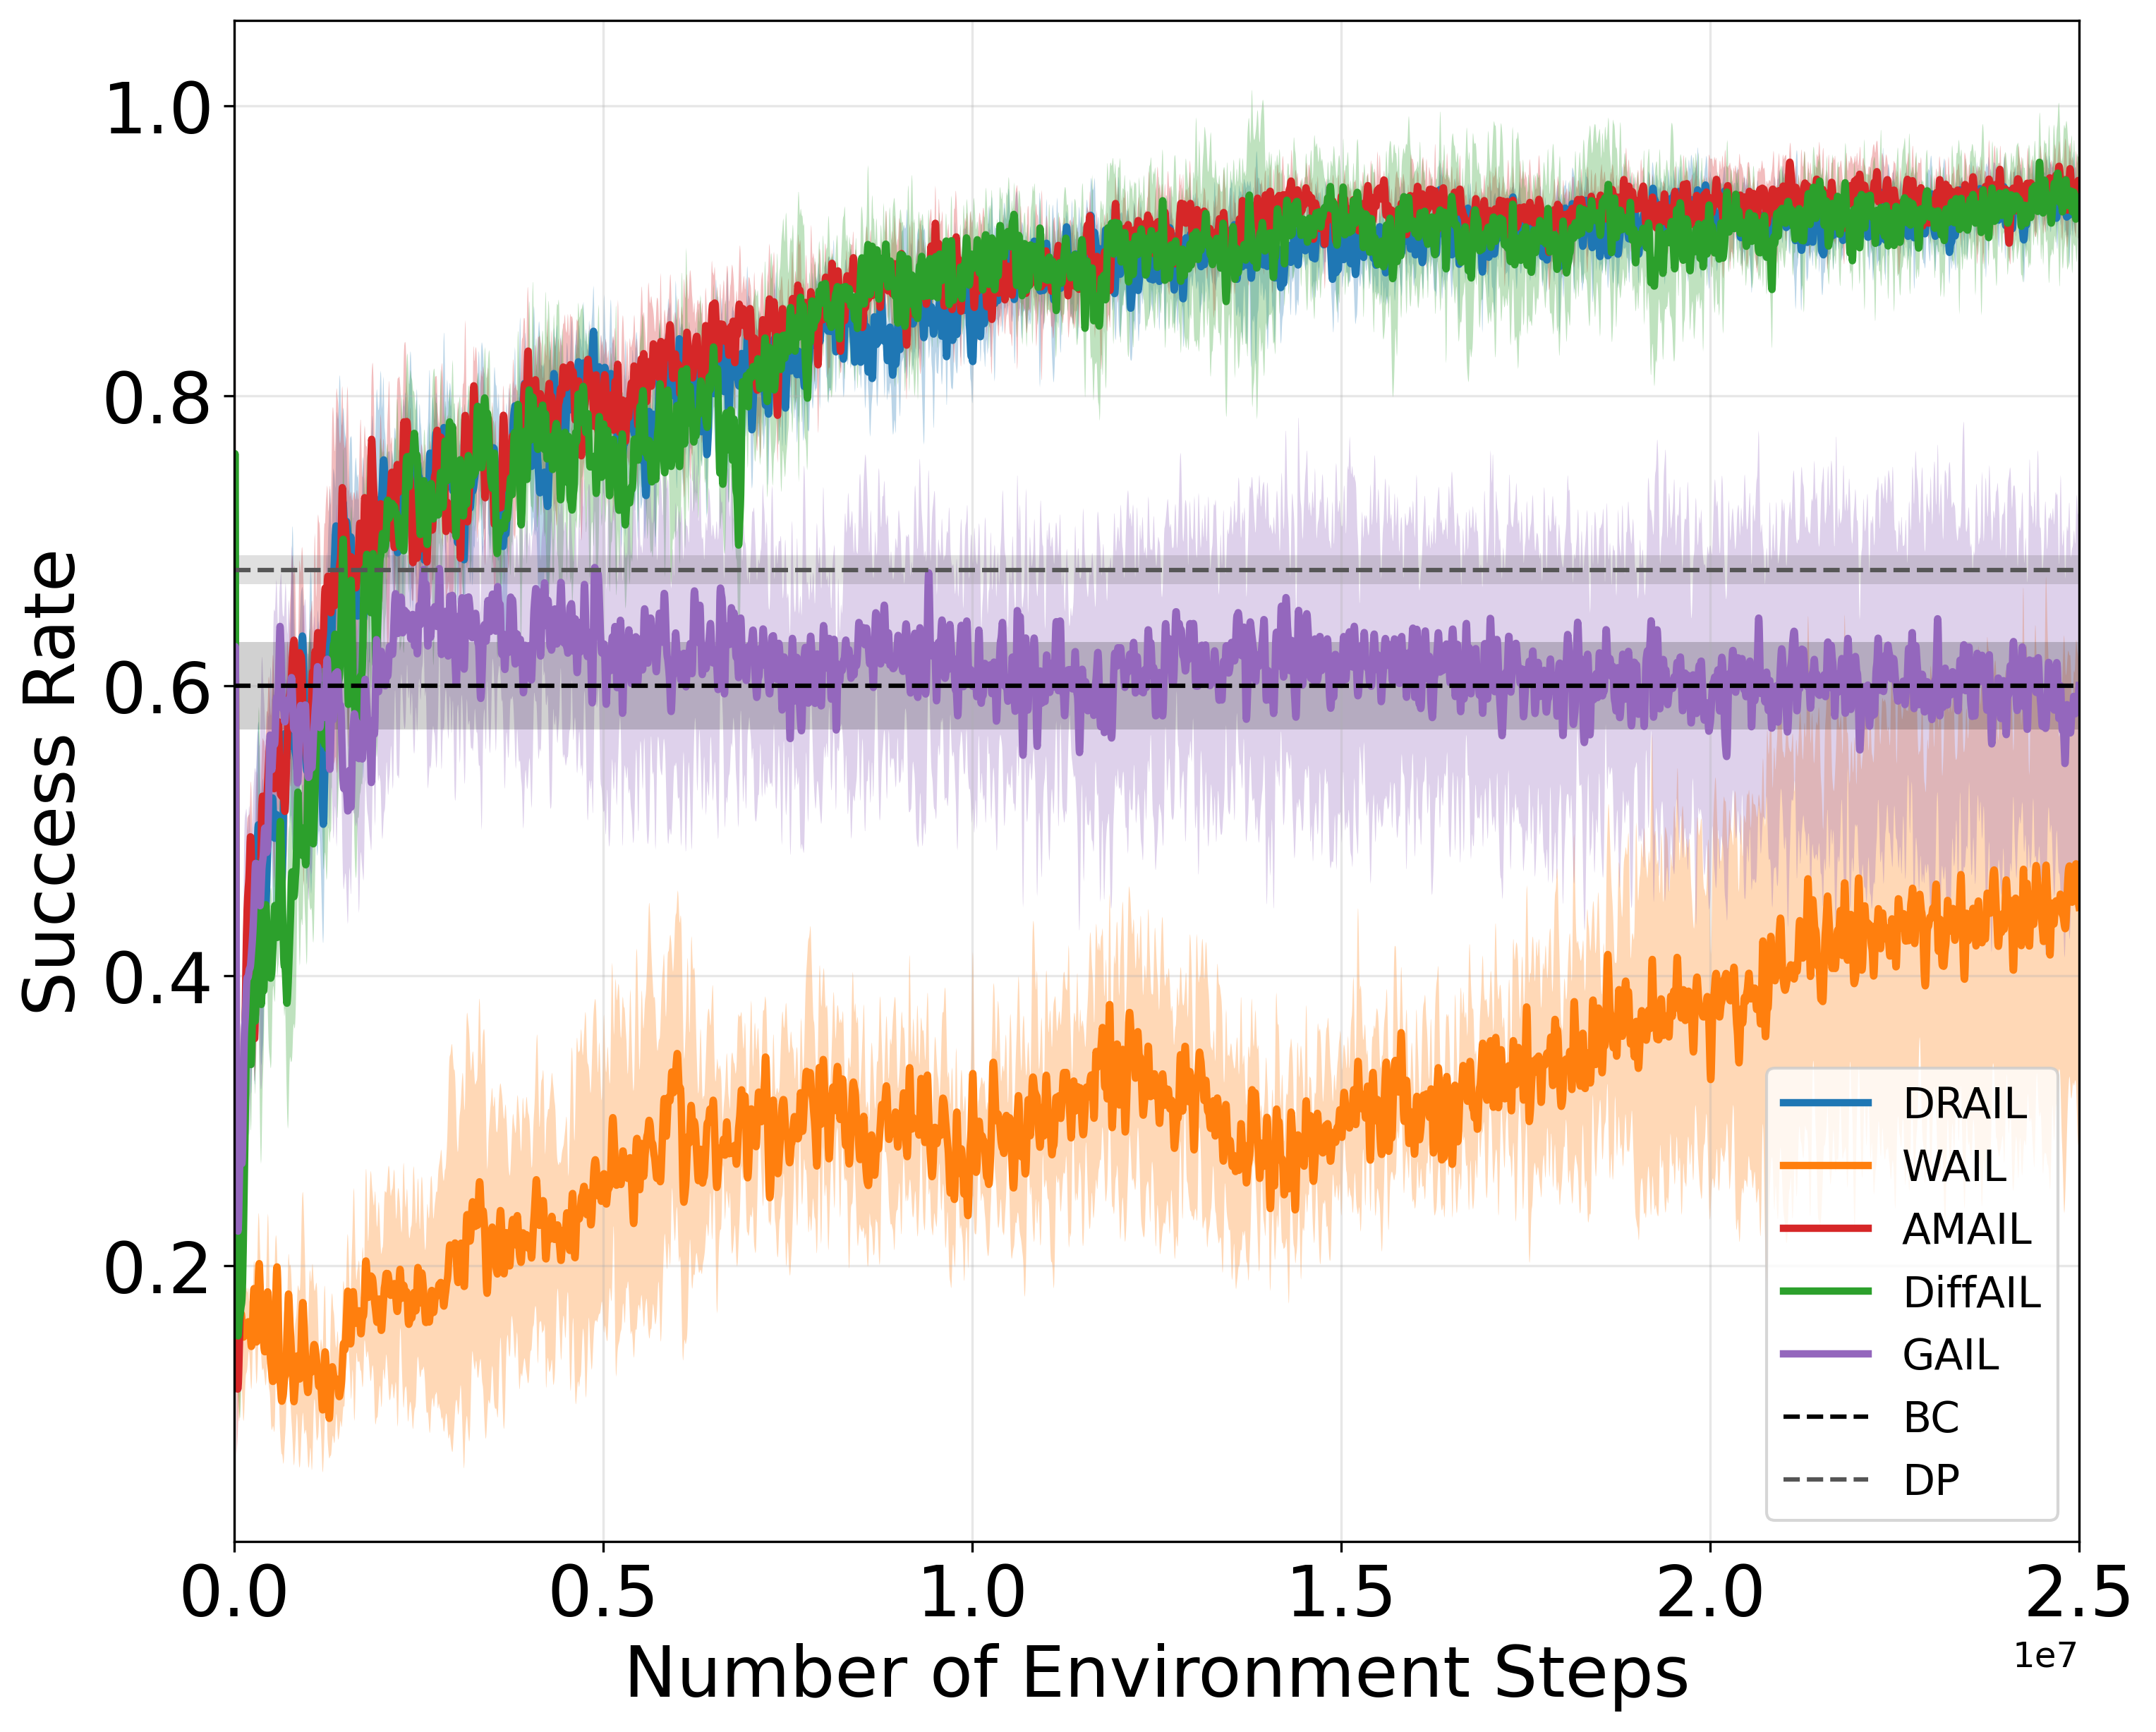
\includegraphics[width=0.33\textwidth]{Maze.png}%
\label{Maze}}%
\hfill
\subfloat[WALKER]{%
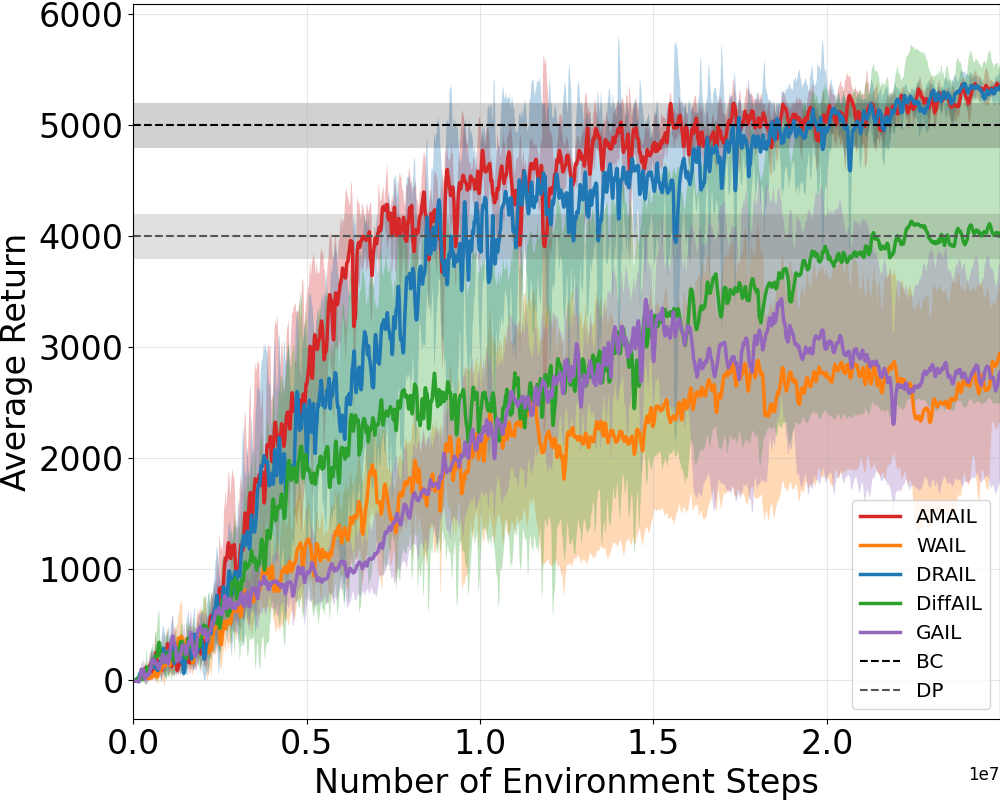
\includegraphics[width=0.33\textwidth]{Walker.png}%
\label{Walker}}%

\caption{\textbf{Learning efficiency}. Our method is compared against six baseline methods across six environments, with each experiment repeated over five random seeds; the curves report mean performance and the shaded regions indicate pointwise standard deviation. Across all tasks and training stages, AMAIL demonstrates faster convergence, reduced variance, and consistently superior performance relative to competing approaches.}
\label{fig_sim2}
\end{figure*}

\subsection{Baselines}
To comprehensively evaluate the effectiveness of AMAIL, we compare it against the following representative imitation learning and adversarial learning baselines:

\textbf{$\bullet$ Behavior Cloning (BC)} is a supervised imitation learning method that directly learns a deterministic or stochastic mapping from states to actions using expert demonstrations. As one of the most fundamental imitation learning approaches, BC serves as a lower-bound baseline, particularly sensitive to covariate shift due to the absence of environment interaction during training.

\textbf{$\bullet$ Diffusion Policy (DP)} models the target policy as a conditional diffusion process. Given a state input and sampled Gaussian noise, the model iteratively denoises the action representation to generate control outputs. As an offline generative policy learning approach, DP is capable of modeling complex, multimodal action distributions.

\textbf{$\bullet$ Generative Adversarial Imitation Learning (GAIL)} formulates imitation learning as a minimax game between a policy generator and a discriminator. The discriminator distinguishes expert trajectories from policy-generated trajectories, while the policy is trained to match the expert's occupancy measure. This framework enables indirect reward learning through adversarial optimization.

\textbf{$\bullet$ Wasserstein Adversarial Imitation Learning (WAIL)} replaces the Jensen-Shannon divergence in GAIL with the Wasserstein distance, leading to smoother gradient signals and improved training stability. By leveraging optimal transport principles, WAIL mitigates reward oscillation and gradient vanishing issues observed in standard adversarial imitation learning.

\textbf{$\bullet$ Diffusion Adversarial Imitation Learning (DiffAIL)} incorporates a diffusion model into the adversarial imitation learning framework. The diffusion loss is integrated into the discriminator's objective, enabling more accurate modeling of the expert data distribution. This enhances the discriminator's capacity to capture complex and high-dimensional action patterns.

\textbf{$\bullet$ Diffusion Rewards Adversarial Imitation Learning (DRAIL)} integrates diffusion-based modeling into the reward learning component of GAIL. By using diffusion processes to characterize the similarity between current states and target states, DRAIL generates smoother and more informative reward signals, thereby alleviating instability commonly observed in adversarial training.



\begin{table*}[!t]
\centering
\caption{Performance Comparison Across Six Tasks}
\label{tab:cluster_tnnls}

\setlength{\tabcolsep}{5pt}
\renewcommand{\arraystretch}{1.1}

\begin{tabular}{
lccccccc
}
\toprule
\multirow{2}{*}{\textbf{Task}} 
& \multicolumn{3}{c}{\textbf{Representative algorithms of imitation learning}} 
& \multicolumn{4}{c}{\textbf{Novel algorithms based on adversarial imitation learning}} \\
\cmidrule(lr){2-4}
\cmidrule(lr){5-8}
& \textbf{BC} & \textbf{DP} & \textbf{GAIL} & \textbf{WAIL} & \textbf{DiffAIL} & \textbf{DRAIL} & \textbf{AMAIL} \\
\midrule

FETCHPUSH & -- & -- & -- & -- & -- & -- & -- \\

FETCHPICK & -- & -- & -- & -- & -- & -- & -- \\

ANTREACH & -- & -- & -- & -- & -- & -- & -- \\

HANDROTATE & -- & -- & -- & -- & -- & -- & -- \\

MAZE & -- & -- & -- & -- & -- & -- & -- \\

WALKER & -- & -- & -- & -- & -- & -- & -- \\

\bottomrule
\end{tabular}
\end{table*}

\begin{figure*}[!t]
\centering

\subfloat[FETCHPUSH]{%
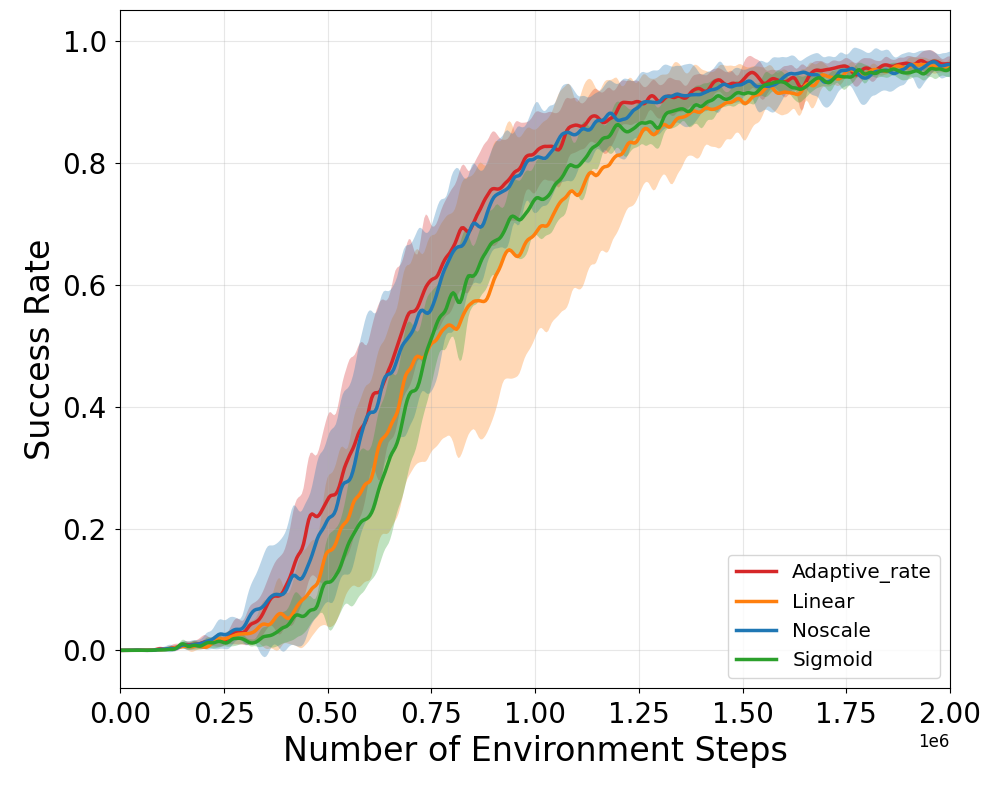
\includegraphics[width=0.33\textwidth]{learning_rate.png}%
\label{The training effects with different weights}}%
\hspace{0.02\textwidth}
\subfloat[Rate]{%
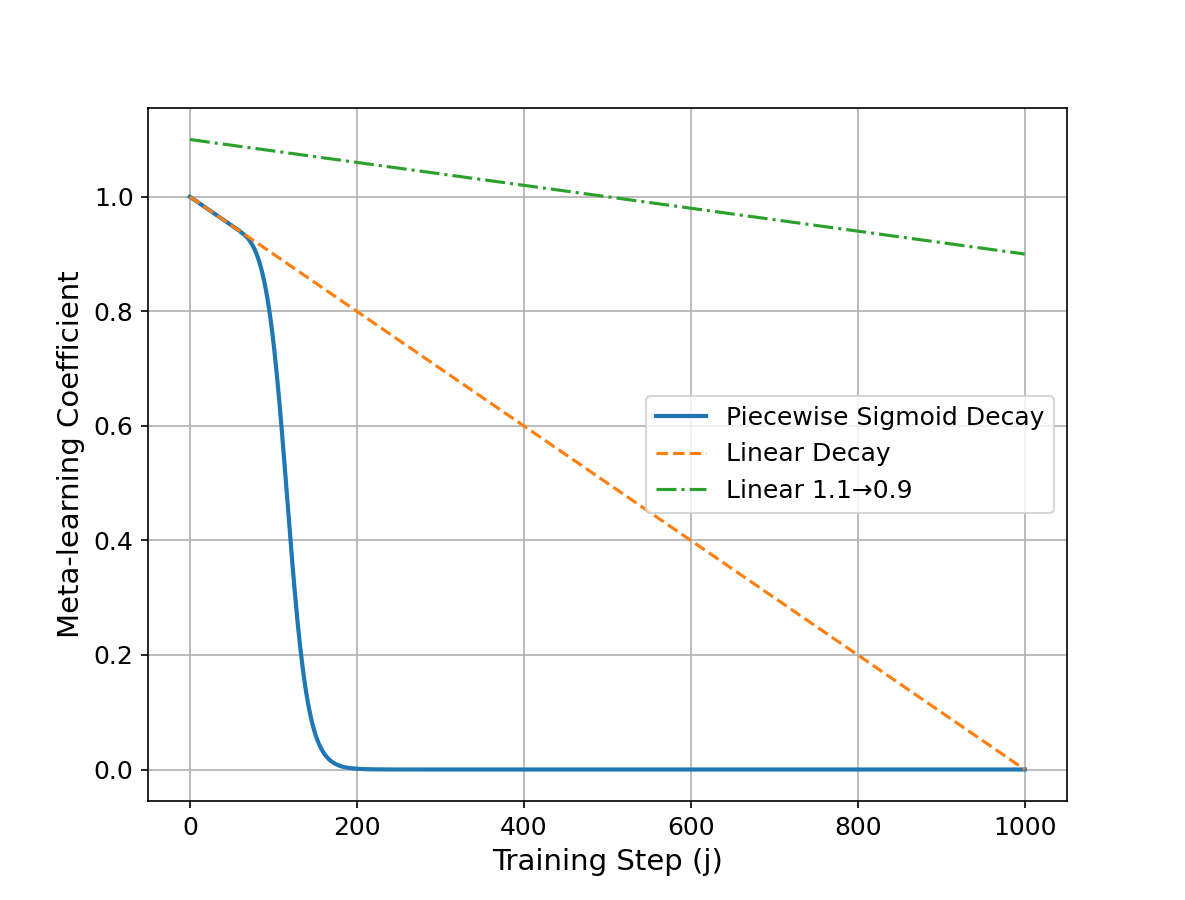
\includegraphics[width=0.38\textwidth]{rate.png}%
\label{rate}}%


\caption{\textbf{Meta-learning Network Coefficient}. The specific parameters of linear attenuation and sigmoid function attenuation have been tested through iteration to obtain the optimal values. Experiments were conducted under the condition of 2.0 times noise in FetchPush. The curve shows that the dynamic weights are superior to the linear weights and sigmoid weights. Scaling can also improve the performance of the model to a certain extent. This is particularly evident when the difference between the output of the meta-learning network and the reinforcement learning objective function value is too large.}
\label{fig_sim3}
\end{figure*}

\subsection{Results and Analysis}
To ensure a systematic and fair evaluation, all methods were trained on expert datasets across six benchmark environments. For each task, experiments were repeated with five independent random seeds, and we report the mean performance and standard deviation to assess both effectiveness and training stability. It is worth noting that Behavior Cloning (BC) and Diffusion Policy are purely offline approaches and therefore do not interact with the environment during training. For comparability, their success rates are plotted as horizontal reference lines in the performance curves.

We first examine learning efficiency under standard expert settings. All models were trained using the complete expert dataset with identical noise conditions (1$\times$, consistent with the expert data collection process). Under these controlled settings, our method achieves performance comparable to or exceeding existing algorithms across all tasks, and demonstrates clear advantages in several environments. In particular, AMAIL improves expert data utilization through meta-learning. On the FETCHPUSH, FETCHPICK, HANDROTATE, and WALKER tasks, it rapidly converges to expert-level performance, indicating that the meta-learning network effectively captures the latent behavioral structure of expert demonstrations and provides meaningful guidance to the policy network. Moreover, performance variance across random seeds is reduced, suggesting that the adaptive learning mechanism enhances robustness to noise and improves generalization. By adopting a two-layer meta-learning architecture, AMAIL extracts high-level structural information from offline demonstrations and transforms it into auxiliary guidance rewards. Unlike conventional imitation learning methods that focus solely on behavior matching, AMAIL models the intrinsic decision logic underlying expert behavior and leverages it to shape policy optimization.

To further investigate the role of meta-guidance, we analyze how to regulate the intervention ratio of the meta-learning network during training. Intuitively, stronger intervention is desirable in the early stages to accelerate representation alignment, while a gradual reduction is beneficial later to avoid over-regularization and performance degradation. In imitation learning, inappropriate intervention can destabilize training or suppress policy improvement. To address this, we use the diffusion discriminator's output to estimate demonstration confidence and dynamically adjust the influence of the meta-learning network on policy updates. We compare this adaptive mechanism with commonly used linear decay and sigmoid decay schedules in the FetchPush environment. Because the magnitude of the meta-learning outputs may differ from reinforcement learning signals, direct combination can lead to under- or over-dominance. Therefore, we rescale the weighted meta-learning outputs to ensure compatibility across tasks and maintain balanced optimization dynamics.

This adaptive control mechanism provides two complementary benefits. First, it encourages efficient exploration by emphasizing high-value behavioral patterns distilled from expert data. Second, it suppresses misleading updates caused by low-confidence or noisy demonstrations. As a result, AMAIL achieves higher data efficiency and stronger robustness, particularly in scenarios with limited or imperfect expert demonstrations.

To further evaluate the robustness and generalization benefits introduced by the adaptive weighting mechanism, we conducted additional experiments on the complete FETCHPUSH dataset under progressively increasing noise levels. Specifically, Gaussian noise was injected into both the initial states and target states of the demonstrations with intensities of 1.25$\times$, 1.75$\times$, and 2.0$\times$ relative to the original data collection setting. This setup simulates blurred or corrupted expert trajectories and forces the models to extract informative behavioral signals from ambiguous state distributions.

As the noise level increased, conventional imitation and adversarial methods suffered significant performance degradation, often accompanied by unstable convergence. Diffusion-based baselines such as DRAIL and DiffAIL demonstrated relatively stronger tolerance to moderate noise due to their generative modeling capability. However, in high-noise regimes, they exhibited slower convergence and eventual performance collapse, primarily because noisy demonstrations weakened the reliability of the learned distributional guidance.

In contrast, AMAIL maintained stable training dynamics and showed minimal degradation in both convergence speed and final performance as noise intensity increased. This robustness stems from the adaptive confidence weighting mechanism, which effectively suppresses the influence of corrupted samples and mitigates systematic bias in the meta-learning network under high-noise conditions. As a result, AMAIL preserves reliable policy improvement even when expert information is substantially perturbed, demonstrating enhanced generalization and anti-noise capability.

\begin{figure*}[!t]
\centering

\subfloat[Noise $\times1.25$]{%
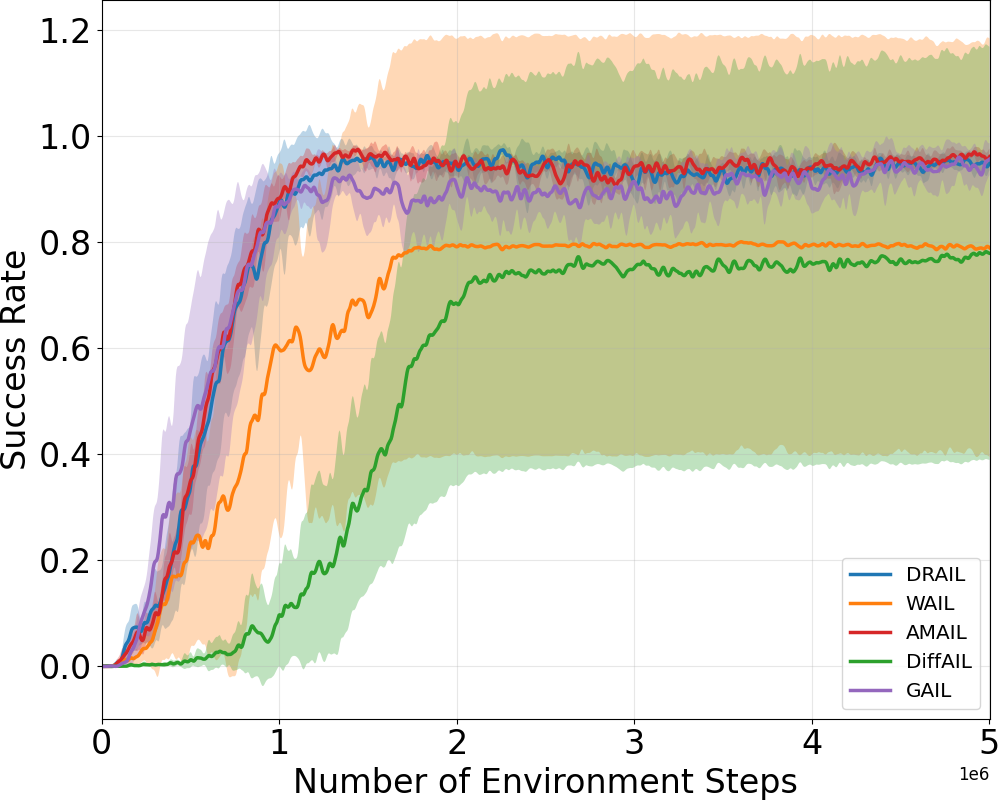
\includegraphics[width=0.33\textwidth]{1.25.png}%
\label{FETCHPUSH 1.25}}%
\hfill
\subfloat[Noise $\times1.75$]{%
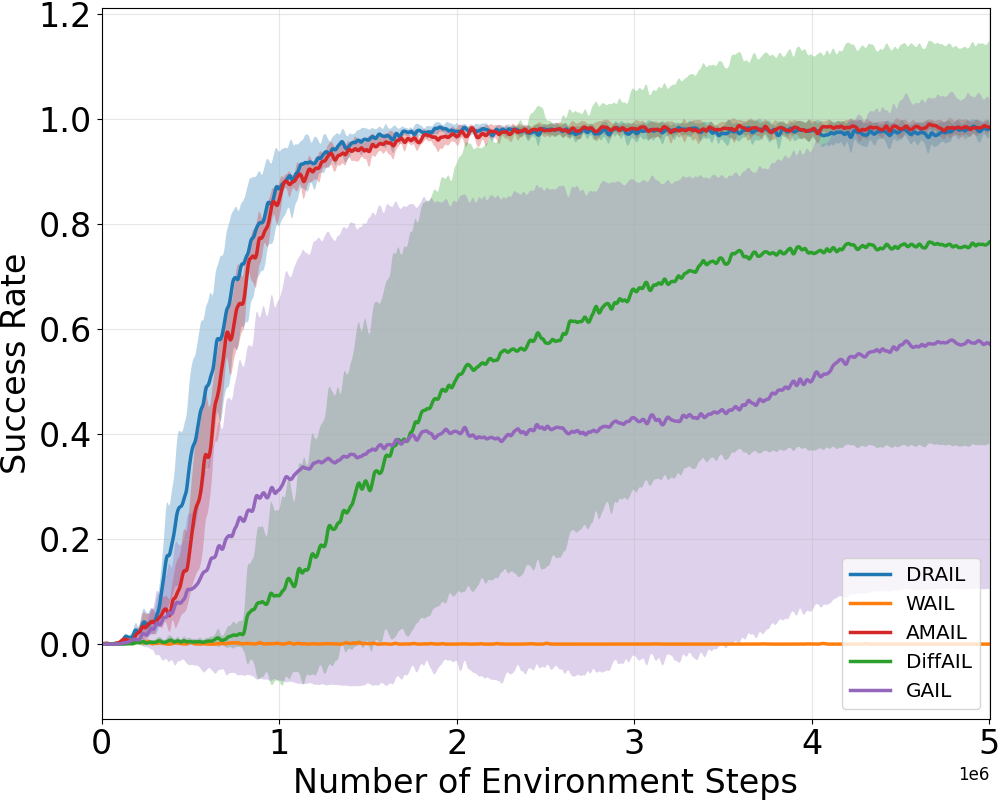
\includegraphics[width=0.33\textwidth]{1.75.png}%
\label{FETCHPUSH x1.75}}%
\hfill
\subfloat[Noise $\times2.00$]{%
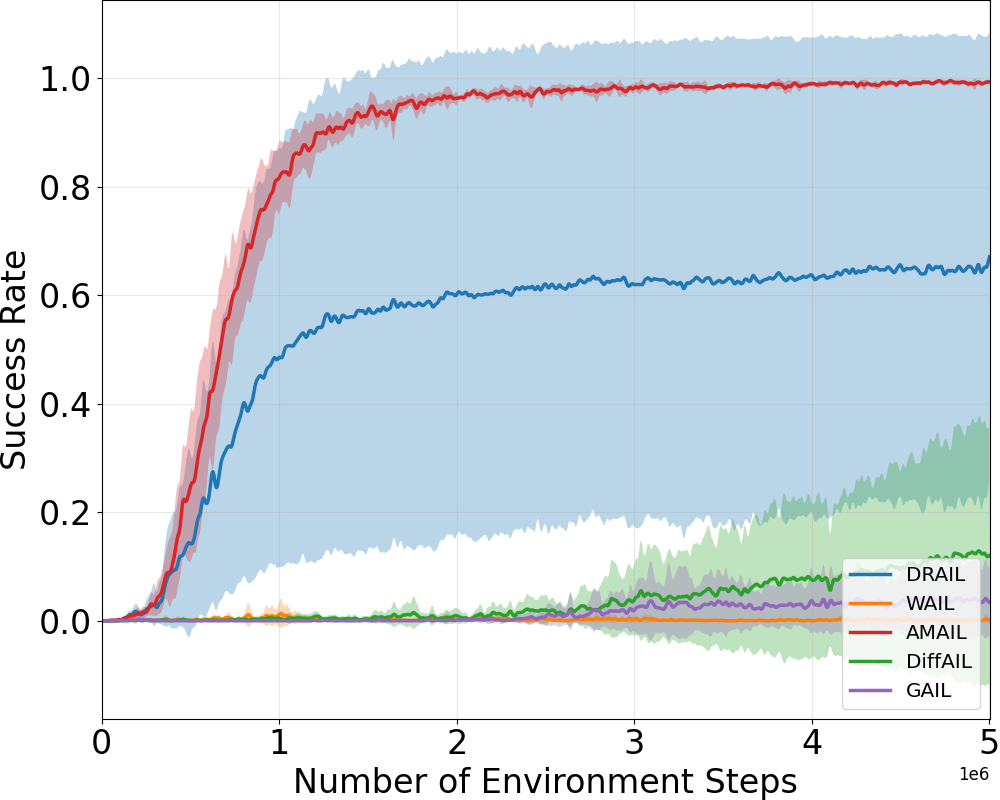
\includegraphics[width=0.33\textwidth]{2.00.png}%
\label{FETCHPUSH x2.00}}%


\caption{\textbf{Noise resistance and generalization ability}. Performance comparison on FETCHPUSH under noise intensities of $\times1.25$, $\times1.75$, and $\times2.00$; curves show mean success rate over five random seeds and shaded regions indicate standard deviation. AMAIL maintains stable convergence and superior final performance as noise increases, demonstrating strong robustness against corrupted expert demonstrations.}
\label{fig_sim4}
\end{figure*}

\section{Conclusion}
This paper introduces Adaptive-Meta Adversarial Imitation Learning (AMAIL), a unified framework that enhances imitation learning through the integration of a meta-learning architecture and a diffusion-based discriminator. The proposed design addresses two central challenges in imitation learning: limited data efficiency and vulnerability to noisy or suboptimal demonstrations. Specifically, we develop an adaptive meta-learning network that captures the intrinsic optimization structure embedded in expert trajectories, enabling rapid and stable policy adaptation. Building upon this foundation, we introduce an adaptive weighting mechanism that leverages diffusion loss to dynamically regulate the influence of meta-learning updates. This mechanism effectively suppresses corrupted or low-confidence samples, thereby improving robustness under distributional perturbations.

Extensive experiments on MuJoCo and PyBullet robotic control benchmarks demonstrate that AMAIL consistently achieves superior learning efficiency, convergence stability, and robustness compared to state-of-the-art baselines. The advantages are particularly pronounced in low-data regimes and high-noise settings, highlighting the effectiveness of the proposed adaptive reweighting strategy and meta-optimization design.

Despite these promising results, the current implementation focuses on low-dimensional state representations. Extending AMAIL to high-dimensional visual observations remains an important direction for future research. One potential avenue is to integrate the proposed adaptive meta-learning mechanism with large-scale perception models, enabling efficient processing of image-based inputs. Moreover, AMAIL's data-efficient learning paradigm could be leveraged to fine-tune pre-trained foundation policies for specialized downstream tasks, thereby accelerating adaptation and improving deployment efficiency in real-world robotic systems.

\begin{thebibliography}{1}
\bibliographystyle{IEEEtran}

\bibitem{ref1}
{\it{Mathematics Into Type}}. American Mathematical Society. [Online]. Available: https://www.ams.org/arc/styleguide/mit-2.pdf

\bibitem{ref2}
T. W. Chaundy, P. R. Barrett and C. Batey, {\it{The Printing of Mathematics}}. London, U.K., Oxford Univ. Press, 1954.

\bibitem{ref3}
F. Mittelbach and M. Goossens, {\it{The \LaTeX Companion}}, 2nd ed. Boston, MA, USA: Pearson, 2004.

\bibitem{ref4}
G. Gr\"atzer, {\it{More Math Into LaTeX}}, New York, NY, USA: Springer, 2007.

\bibitem{ref5}M. Letourneau and J. W. Sharp, {\it{AMS-StyleGuide-online.pdf,}} American Mathematical Society, Providence, RI, USA, [Online]. Available: http://www.ams.org/arc/styleguide/index.html

\bibitem{ref6}
H. Sira-Ramirez, ``On the sliding mode control of nonlinear systems,'' \textit{Syst. Control Lett.}, vol. 19, pp. 303--312, 1992.

\bibitem{ref7}
A. Levant, ``Exact differentiation of signals with unbounded higher derivatives,''  in \textit{Proc. 45th IEEE Conf. Decis.
Control}, San Diego, CA, USA, 2006, pp. 5585--5590. DOI: 10.1109/CDC.2006.377165.

\bibitem{ref8}
M. Fliess, C. Join, and H. Sira-Ramirez, ``Non-linear estimation is easy,'' \textit{Int. J. Model., Ident. Control}, vol. 4, no. 1, pp. 12--27, 2008.

\bibitem{ref9}
R. Ortega, A. Astolfi, G. Bastin, and H. Rodriguez, ``Stabilization of food-chain systems using a port-controlled Hamiltonian description,'' in \textit{Proc. Amer. Control Conf.}, Chicago, IL, USA,
2000, pp. 2245--2249.

\end{thebibliography}


\newpage

% \section{Biography Section}
% If you have an EPS/PDF photo (graphicx package needed), extra braces are
%  needed around the contents of the optional argument to biography to prevent
%  the LaTeX parser from getting confused when it sees the complicated
%  $\backslash${\tt{includegraphics}} command within an optional argument. (You can create
%  your own custom macro containing the $\backslash${\tt{includegraphics}} command to make things
%  simpler here.)
 
% \vspace{11pt}

% \bf{If you include a photo:}\vspace{-33pt}
% \begin{IEEEbiography}[{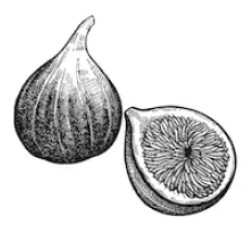
\includegraphics[width=1in,height=1.25in,clip,keepaspectratio]{fig1}}]{Michael Shell}
% Use $\backslash${\tt{begin\{IEEEbiography\}}} and then for the 1st argument use $\backslash${\tt{includegraphics}} to declare and link the author photo.
% Use the author name as the 3rd argument followed by the biography text.
% \end{IEEEbiography}

% \vspace{11pt}

% \bf{If you will not include a photo:}\vspace{-33pt}
% \begin{IEEEbiographynophoto}{John Doe}
% Use $\backslash${\tt{begin\{IEEEbiographynophoto\}}} and the author name as the argument followed by the biography text.
% \end{IEEEbiographynophoto}




\vfill

\end{document}


